\part{L'apprentissage machine au c\oe ur de l'acquisition des données}

\begin{figure}[ht]
    \centering
    \caption{Processus de travail d'encodage}
    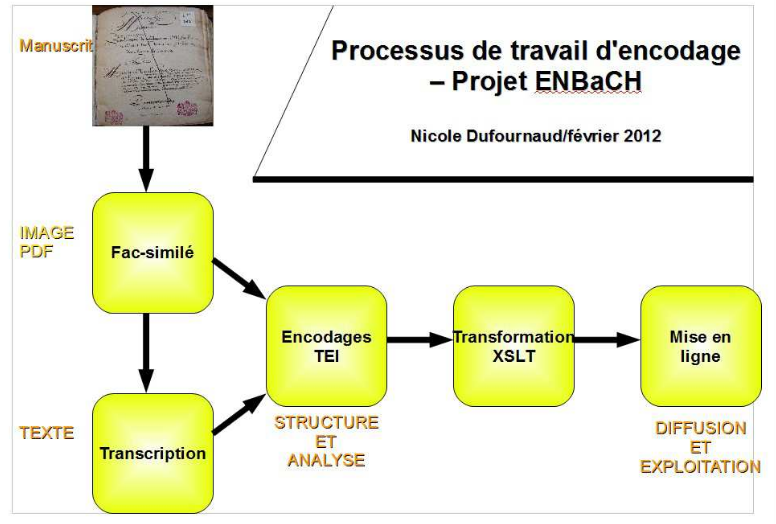
\includegraphics[width=16cm]{images/processus_encodage.png}
    \label{processus_encodage}
\end{figure}

La suite de ce mémoire va être consacrée à l'acquisition et au traitement des données. Nous avons trouvé ici un schéma qui éclaire en partie le processus qui amène à la mise en ligne des données. Même si celui-ci diffère selon les projets, on observe de grandes constantes.

Tout d'abord, il y a la donnée brute~: le manuscrit. C'est le cas pour le projet Le Play. Pour ELICOM, nous avons à faire à une édition papier imprimée. Après le manuscrit suit l'image numérisée, dont on se sert pour faire les transcriptions - c'est la partie acquisition des données - et à partir de là, l'encodage en TEI. On peut avoir recours à une transformation XSLT (\emph{Extensible Stylesheet Language Transformations}), on parlera rapidement de cette éventualité. Et enfin, la mise en ligne, objectif de nos projets pour leur diffusion et exploitation. Puisse ce schéma éclairer les propos qui suivront. 

\chapter{L'apprentissage machine}

\section{Petite histoire de l'apprentissage machine}

Pour mieux comprendre ce qui va suivre, il importe de revenir sur ce qu'est l'apprentissage machine afin de mieux saisir en quoi il intéresse nos projets.

Le terme \emph{Machine Learning} (ML), traduit en français par \inquote{apprentissage machine} ou encore \inquote{apprentissage automatique}, est apparu pour la première fois dans la bouche d'Arthur Samuel, en 1959, un pionnier américain dans le domaine des jeux vidéo et de l'intelligence artificielle. Il évoque la possibilité qu'a la machine d'apprendre sans être vraiment programmée\footnote{\emph{An introduction to Machine Learning}, Site web GeeksforGeeks, URL~: \url{https://www.geeksforgeeks.org/introduction-machine-learning/} (visité le 20/09/2020). }.

En effet, la machine peut être programmée pour apprendre de son expérience. On verra très nettement par la suite qu'elle fait, pour ainsi dire, des progrès. Elle apprend une écriture, à travers des \inquote{\emph{features\footnote{Une des techniques de reconnaissance est la \inquote{classification par caractéristiques (\emph{features}) : une forme à reconnaître est représentée par un vecteur de valeurs numériques - appelées \emph{features} en anglais - calculées à partir de cette forme}. Voir \emph{Reconnaissance optique de caractères}, Wikipedia, URL : \url{https://fr.wikipedia.org/wiki/Reconnaissance_optique_de_caracteres} (visité le 30/09/2020).}}}, et plus on lui donne de lettres à apprendre, plus elle progresse, jusqu'à pouvoir faire la transcription elle-même en prédisant le caractère à reconnaître par rapport à ce qu'elle a appris, avec un taux de réussite plus ou moins important\footnote{L'apprentissage machine a plusieurs divisions comme l'apprentissage supervisé ou non supervisé, ou encore l'apprentissage par renforcement et l'apprentissage semi-supervisé. Mais nous ne rentrons pas ici dans les détails de l'algorithme.}. 

\section{Apprentissage machine et intelligence artificielle}

Comme nous l'avons rapidement souligné, l'apprentissage machine est une composante de l'intelligence artificielle (IA). Celle-ci est la \inquote{recherche de moyens susceptibles de doter les systèmes informatiques de capacités intellectuelles comparables à celles des êtres humains}\footnote{\emph{La Recherche}, janv. 1979, n.96, vol. 10, p. 61}. Elle se traduit par  « l'ensemble des théories et des techniques mises en œuvre en vue de réaliser des machines capables de simuler l'intelligence »\footnote{\emph{Intelligence artificielle}, Wikipédia, URL~: \url{https://fr.wikipedia.org/wiki/Intelligence_artificielle} (visité le 20/09/2020).}. C'est une capacité d'un programme informatique à fonctionner comme un cerveau humain. Elle utilise, avec les réseaux de neurones la façon de fonctionner de l'intelligence humaine. Ainsi, on voit que le fait qu'une machine puisse apprendre et faire en quelque sorte des progrès fait partie de l'IA. Le schéma ci-dessous\footnote{Gauthier Poupeau, \emph{Open Data, Big data, Data Mining,}Module data, M2 TNAH ENC, Cours 2, 21 octobre 2019} permet de comprendre davantage la place du \emph{Machine Learning} dans l'IA. On voit que l'apprentissage machine et l'apprentissage profond ou \emph{deep learning} sont des sous-ensemble de l'IA. Cependant, ils ne sont pas l'IA mais un moyen de parvenir à l'IA un jour. 

\begin{figure}[ht]
    \centering
    \caption{\emph{Machine learning} et IA}
    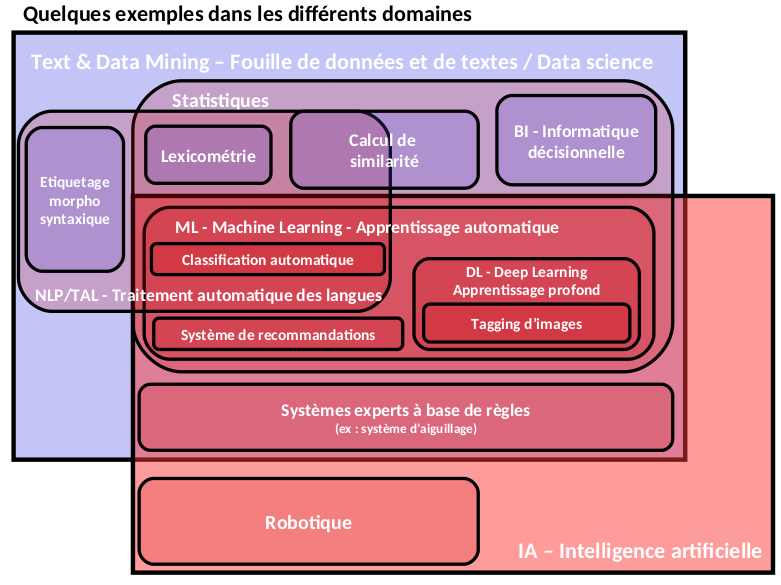
\includegraphics[width=16cm]{images/ia_poupeau.png}
    \label{ia_poupeau}
\end{figure}


Ainsi, pour distinguer \emph{machine learning} et \emph{deep learning}, on peut dire que le \emph{machine learning} est un \inquote{système visant à accomplir des tâches à partir de caractéristiques et attributs communs (patterns) ``appris'' dans un ensemble de données d'exemples}\footnote{\emph{Idem}, p. 27}~: la machine apprend les données et les applique de la bonne façon ; tandis que le \emph{deep learning} est un sous-ensemble du \emph{machine learning}, une \inquote{technique d’apprentissage cherchant à reproduire le mécanisme des réseaux de neurones du cerveau humain}\footnote{\emph{Ibidem.} p. 28}. Il est plus poussé, plus abouti et plus autonome\footnote{Voir \emph{Artificial intelligence vs Machine Learning vs Deep Learning}, Site web Geeksforgeeks, URL~: \url{https://www.geeksforgeeks.org/artificial-intelligence-vs-machine-learning-vs-deep-learning/?ref=rp} (visité le 20/09/2020).}.

Ainsi, nous verrons que les technologies que nous utiliserons de \emph{machine learning} ne sont pas encore abouties et nécessiteront un traitement conséquent. 

\section{L'apprentissage machine dans nos deux projets}

Lorsqu'on a une quantité de lettres à éditer de façon numérique, comment utiliser au mieux les capacités de la machine pour qu'elle nous aide dans l'acquisition des données ?
C'est tout le rôle de l'apprentissage machine qui permet une reconnaissance automatique des caractères et permet la transcription des textes. Or, nous sommes ici face à deux types de textes~: pour ELICOM, nous avons des éditions papier numérisées et disponibles sur Gallica, qui ont été imprimées. Ce sont des caractères d'imprimerie. Pour l'édition numérique de la correspondance de Frédéric Le Play, ce sont des manuscrits écrits au moins de moitié si ce n'est majoritairement de la main de Le Play. Ce sont donc des caractères d'écriture manuscrite. À chaque projet corrrespond donc une technologie différente. Pour les caractères d'imprimerie, on parlera d'\emph{Optical Character Recognition} ou Reconnaissance optique de caractères (OCR), pour la reconnaissance de l'écriture manuscrite, on parlera d'\emph{Handwritten Text Recognition} (HTR). \\

Ainsi, l'OCR\begin{quote}
    \inquote{désigne le processus informatique qui vise à transposer des éléments textuels présents sur une image numérique vers un fichier de texte de manière automatique. Il s'agit, en d'autres termes, de faire réaliser par l'ordinateur la tâche de copie du texte\footnote{Alix Chagué, \emph{Constituer un corpus pour la fouille de texte - de la transcription des documents d’archives à l’annotation~: exploration d’une méthodologie par l’ANR Time Us}, mémoire de master « Technologies numériques appliquées à l’histoire », dir. Vincent Jolivet et Éric de la Clergerie, École nationale des
chartes, 2018, p.41.}.
}
\end{quote}

L'OCR de Gallica est un service qui permet la reconnaissance de texte dans une image\footnote{\emph{Mode texte et OCR}, Site web BNF.Gallica, URL~: \url{https://gallica.bnf.fr/edit/und/consulter-les-documents} (visité le 21/09/2020).}. Ainsi, le contenu des documents numérisés est extrait et transformé en fichier texte. Gallica propose le téléchargement au format \citecode{.txt} du résultat de l'OCR. Néanmoins, il ne s'agit pas de texte brut mais d'un texte semi-structuré via des balises \emph{Hypertext Markup Language} (HTML), langage de balisage conçu pour représenter les pages web. Le texte étant ainsi structuré par les balises, on peut ensuite le transformer plus facilement en vue de notre édition. Nous y reviendrons. Le service de Gallica a donc été très précieux pour notre projet d'ELICOM. \\ 

Quant à l'édition numérique de la correspondance de Frédéric Le Play, nous nous sommes servie de l'HTR via Transkribus, qui permet de transcrire cette fois l'écriture manuscrite, grâce à l'entraînement d'un modèle par main. \\

Ainsi, l'apprentissage machine est au c\oe ur de l'acquisition des données pour nos deux projets. Il est temps de voir cela plus en détail, avec l'OCR et l'HTR.



\chapter{L'OCR de Gallica}

\section{Un service à ne pas négliger}
\subsection{Un OCR plutôt fiable}
Pour le projet ELICOM du Labex OBVIL, nous avons beaucoup exploité l'OCR de Gallica.
En effet, les textes que nous avons extraits sont issus d'un traitement OCR brut, sans relecture, que nous relirons sommairement par la suite. La qualité (taux OCR) dépend de l'état de la source, de la langue, mais aussi de la campagne de numérisation\footnote{C'est la même chose que pour le projet de la Très grande bibliothèque (TGB) mené aussi par OBVIL, voir~: \emph{TGB (BnF – OBVIL)}, Site web provisoire TGB, OBVIL et BNF, URL~: \url{http://obvil.lip6.fr/tgb/} (visité le 08/09/2020).}. Certains livres numérisés avaient par exemple des marques de crayon de papier, ce qui est parfois mal interprété par l'OCR. 
En effet, \begin{quote}
    \inquote{Même si les techniques d'OCR sont en progrès constant, la qualité de reconnaissance dépend malgré tout d'un grand nombre de facteurs liés tant au document original qu'à la numérisation elle-même. Ainsi les documents patrimoniaux de Gallica présentent un certain nombre de défis pour l’OCR~: dégradation du papier ou de l’encrage, polices de caractères ou orthographes anciennes, etc. De plus, les anciens modes de numérisation (en noir et blanc, d’après microfilm) ont un impact négatif sur les performances\footnote{\emph{Mode texte et OCR}, Site web BNF.Gallica, URL~: \url{https://gallica.bnf.fr/edit/und/consulter-les-documents} (visité le 21/09/2020).}.}
\end{quote}
Certains textes ont cependant un taux avancé d’OCR de 100\%. Cependant, un taux de 100\% ne signifie pas un sans fautes. De toutes façons, une relecture précise et attentive sera toujours nécessaire même sur un texte dont le taux est déclaré de 100\%. 
En effet, 
\begin{quote}
    \inquote{Ces estimations donnent généralement un bon aperçu de la qualité globale d’un document, mais elles ne doivent pas être confondues avec le taux qualité réel,  qui ne peut être connu (sauf à corriger le texte d’un document et comparer cette référence avec le texte OCR, ce qui est impossible dans un contexte de numérisation de masse).
De plus, ces indicateurs ne sont pas toujours calculés à partir de la totalité du document ; il se peut par exemple que des zones illisibles ou trop complexes soient exclues du calcul et que la qualité perçue par le lecteur soit ainsi très nettement inférieure à la qualité annoncée\footnote{\emph{Idem.}.}}
\end{quote}

L'avantage que représentent les imprimés du XIX\up{e} siècle est leur relative modernité~: ils sont à la fois suffisamment anciens pour être libres de droits, contrairement aux imprimés des XX\up{e} et XXI\up{e} siècle, et ils ont aussi l'avantage d'être relativement modernes dans leur typographie, donc mieux reconnus automatiquement que les imprimés plus anciens qui comportent souvent des \inquote{s} longs ou autres caractéristiques qui sont autant d'obstacles pour l'OCR et nuisent à sa qualité.

Comme nous l'avions souligné lors de la présentation des sources\footnote{Voir 3.2}, nous avons choisi les correspondances à traiter en priorité d'une part en fonction des marqueurs du texte qui garantissent une extraction plus aisée, d'autre part en fonction de la qualité de l'océrisation. 
Or, la correspondance d'Alphonse de Lamartine semblait réunir ces deux avantages~: pour ce qui est de l'extraction, elle était classée \inquote{relativement facile grâce aux chiffres romains qui délimitent les lettres} dans le cahier des charges, et l'OCR de Gallica indiquait un taux de réussite estimé à 100\%. Nous avons donc choisi de commencer par là notre travail d'extraction et d'acquisition des données. Puis nous nous sommes concentrée sur la correspondance de Félicité de Lamennais pour finir ensuite sur celle de Pierre-Joseph Proudhon. 

Une question s'est posée assez rapidement~: devons-nous systématiquement utiliser le service OCR de Gallica ou est-il opportun de passer par un autre moyen pour extraire le texte, comme par exemple Transkribus ou un équivalent. Nous avons donc demandé conseil à des personnes expertes en la matière. À cela il nous a été répondu que l'OCR de Gallica est un service à ne pas négliger, et comme vu plus haut, les taux de réussite étant relativement bons, il nous a paru plus intéressant de l'exploiter au maximum, d'autant que nous ne sommes pas intéressés par une correspondance entre l'image et le texte, étant donné que nous ne mettrons en ligne que le texte extrait et non l'image de la première édition papier. 

Revenons donc sur cette phase d'acquisition et de pré-traitement des données. Celle-ci s'est faite en plusieurs étapes. 

\subsection{Extraction de l'OCR en HTML}

Pour acquérir les données, il s'agit de les extraire. Cela a occupé la première phase de notre travail. 
Pour chacun des auteurs sélectionnés, nous sommes allés sur le catalogue général de la BNF qui nous a redirigé vers la page de Gallica permettant de télécharger la correspondance sous trois formats~: soit PDF (\emph{Portable Document Format}), soit JPEG (\emph{Joint Photographic Experts Group}), ou encore TXT (fichier texte). Nous avons choisi cette dernière option. En téléchargeant l'OCR en fichier texte brut.
En effet, cela permet d'une part de s'assurer de la qualité de l'océrisation~: au début de chaque fichier TXT extrait se trouve un récapitulatif sur le document et ses métadonnées essentielles, et une phrase générée automatiquement elle aussi donnant des précisions sur l'OCR. Ainsi, pour la correspondance de George Sand, on peut lire que \inquote{Le texte affiché peut comporter un certain nombre d'erreurs. En effet, le mode texte de ce document a été généré de façon automatique par un programme de reconnaissance optique de caractères (OCR). Le taux de reconnaissance estimé pour ce document est de 96~\%.} L'OCR est ici brute~: elle n'a pu être relue. Ces erreurs sont repérées par des caractères gris pâles au lieu des caractères noirs.

\begin{figure}[ht]
    \centering
    \caption{L'OCR de George Sand sous format TXT}
    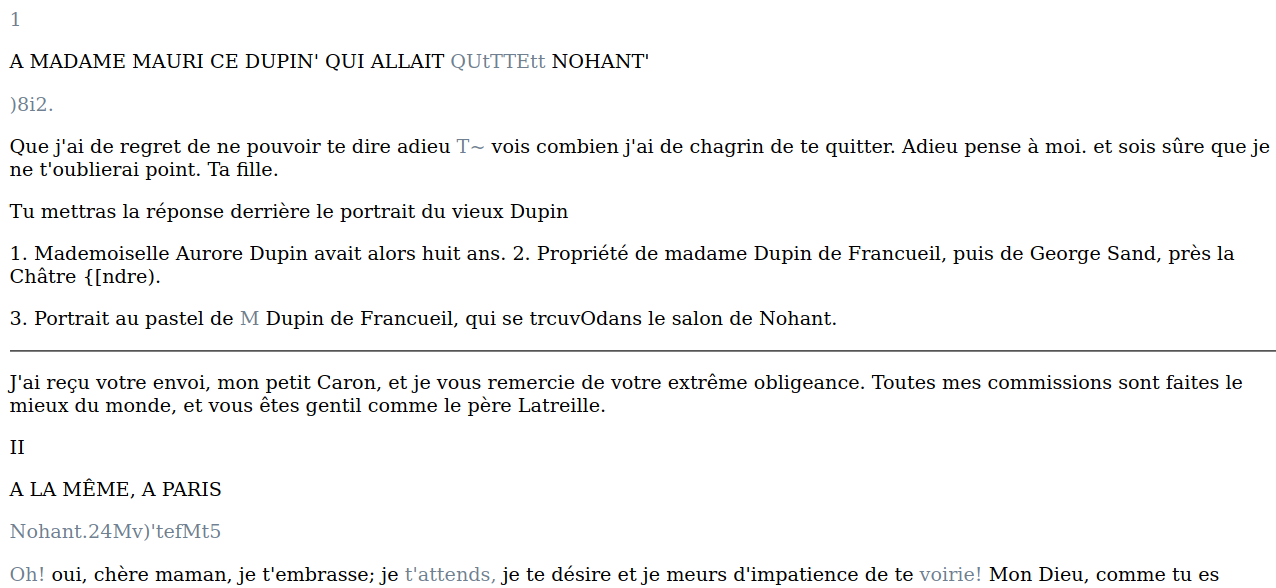
\includegraphics[width=16cm]{images/sand-ocr.png}
    \label{sand-ocr}
\end{figure}

Ainsi, pour le premier volume de la correspondance de George Sand\footnote{\emph{Correspondance~: 1812-1876. George Sand}, BNF.Gallica, URL~: \url{https://gallica.bnf.fr/ark:/12148/bpt6k2065433/f1n385.texteBrut} (visité le 19/05/2020).}, on constate ici des mots grisés~: ce sont toutes les mots soupçonnés d'avoir été mal lu par la reconnaissance automatique. La machine indique donc qu'elle estime s'être trompée sur ces parties. Et effectivement, on peut lire qu'il est écrit \inquote{)8i2.} au lieu de \inquote{1812}, ou encore \inquote{T~} au lieu de \inquote{Tu}. 
Cependant, on voit aussi que certaines parties en noir, et donc présumées justes, sont en réalité fausses~: ainsi il est écrit \inquote{\{[ndre)} au lieu de \inquote{(Indre)}~: la parenthèse ouvrante a été remplacée par une accolade ouvrante, et le \inquote{I} majuscule a été remplacé par un crochet ouvrant. On a donc ici une illustration des limites de l'OCR.

Mais que faire avec ce texte brut ? Il ne nous intéresse pas particulièrement. Il s'agit donc d'extraire le code source sous le format HTML. 

HTML est le langage informatique de base d'Internet, utilisé pour la mise en forme des pages Web\footnote{Depuis 2014, on en est à la version HTML5. Voir~: \emph{HTML (HyperText Markup Langage)~: définition, traduction}, Site web JDN, URL~: \url{https://www.journaldunet.fr/web-tech/dictionnaire-du-webmastering/1203255-html-hypertext-markup-langage-definition-traduction/} (visité le 21/09/2020).}. Il repose sur un système de balises, d'où son nom qui signifie \inquote{langage de balisage d'hypertexte}. 
Comme pour XML, les balises vont toujours par deux, une ouvrante (pour un paragraphe, ce sera \citecode{<p>}), une fermante (\citecode{</p>}).
 La balise ouvrante peut avoir un attribut pour qualifier l'élément.

En extrayant l'OCR sous le format HTML, l'avantage est d'avoir un texte déjà structuré. On peut le constater ci-dessous avec l'exemple de l'OCR de Lamartine au format HTML, avec l'éditeur XML Oxygen XML Editor. Chaque part de texte signifiant - comme la ligne de la date, le salut, le paragraphe - est encadré par une balise \citecode{<p>} indiquant que c'est un paragraphe ou du moins une division particulière. Par ailleurs, les métadonnées sont comprises dans une balise \citecode{head}, elle-même embrassant des balises \citecode{<meta>} contenant des attributs comme \citecode{@name} ou \citecode{@content}.
Le corps du texte quant à lui est contenu dans une balise \citecode{<body>}. Les balises \citecode{<span>} indiquent les erreurs de l'OCR.

\begin{figure}[ht]
    \centering
    \caption{L'OCR de Lamartine en HTML sous Oxygen XML Editor}
    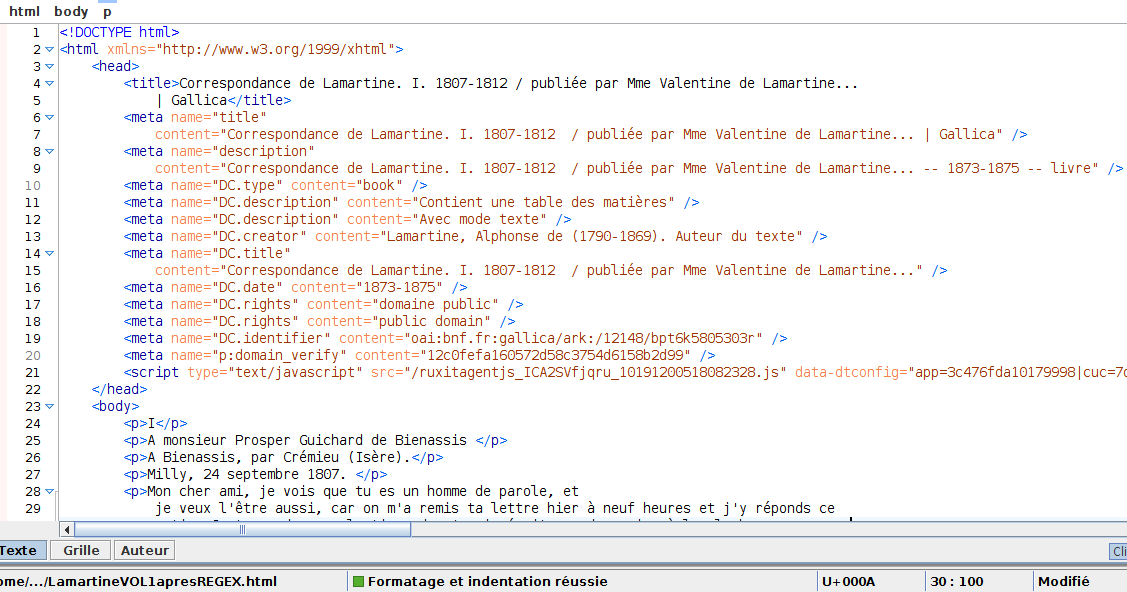
\includegraphics[width=16cm]{images/lamartine_html.png}
    \label{lamartine_html}
\end{figure}

Le texte est donc bel et bien structuré et cela nous permettra par la suite de le transformer plus facilement en XML. En attendant, l'OCR extrait en HTML est loin d'être parfait. L'illustration présente (figure 8.2) montre l'HTML tel qu'il est après correction. En effet, toute une phase de pré-traitement s'est avérée être nécessaire avant de passer à l'étape de transformation en XML que nous développerons dans la quatrième partie de notre mémoire.


\section{Un pré-traitement qui suscite des questionnements}

\subsection{Rendre l'HTML valide et bien indenté}

Notre premier souci lors du téléchargement de l'OCR en HTML a été de vérifier la validité et la bonne indentation de notre fichier HTML. Or, les différents fichiers extraits de Gallica présentaient tous des erreurs dans les balises~: les balises \citecode{<meta>} n'étaient pas fermées et il était donc impossible d'indenter le texte correctement. De même pour les balises \citecode{<br>} (élément de saut de ligne) et \citecode{<hr>} (pour \emph{horizontal rule}, règle horizontale servant de séparation, elles indiquent ici les changements de page, on en trouve donc 391 occurences pour Lamartine). Nous avons donc commencé par fermer toutes ces balises\footnote{Avec la nouvelle version d'Oxygen XML Editor, cela peut se faire de façon automatique.}. Nous avons également choisi de supprimer les ensembles de balises \citecode{</p><hr/><p>} (40 occurences dans Lamartine) et \citecode{</p><p>} (58 occurences dans Lamartine) quand elles divisaient des phrases, étant donc inopportunes et rompant par là l'unité. De même, les titres courants, figurant en en-tête sont des informations superflues. Fort heureusement, elles ont été supprimées automatiquement par l'OCR pour la correspondance de Lamennais (en effet, on lisait « CORRESPONDANCE » à la page de gauche, « DE LAMENNAIS » à la page de droite), ne polluant donc pas l’HTML, contrairement à Lamartine où l'OCR de Gallica ne les avait pas supprimés.

Ensuite, même si cela n'était pas absolument nécessaire, nous avons supprimé tout ce qui concernait les rappels de la demande, les tables des matières et préfaces. Nous aurions aussi pu le faire en amont, lors du téléchargement.
Ainsi, l’HTML de Lamennais comporte 12 204 lignes au départ, 8680 après nettoyage (soit le double de l’HTML de Lamartine après nettoyage). 

Nous avons donc désormais un HTML valide et bien indenté. Cependant, des fautes subsistent.

\subsection{Quelques fautes de l'OCR, visibles dans l'HTML}

Nous avons vu plus haut que certaines fautes étaient grisées dans l'OCR en format TXT. Ceci se retrouve donc logiquement dans l'OCR en format HTML, avec les balises \citecode{<span>}. Or, on remarque que celles-ci sont parfois utilisées à bon escient, tandis que d'autres fois, elles sont absentes ou superflues.

Les balises \citecode{<span>} indiquant les doutes sur l’OCR sont absentes dans la correspondance de Lamartine. En revanche, on en trouve 510 ouvrantes et fermantes dans le premier volume de correspondance de Lamennais. C'est pour les erreurs quasiment avérées, mais beaucoup d’autres erreurs se sont glissées dans le texte, sans être signalées par une balise.  Une relecture sera donc nécessaire. 
Ainsi, à la ligne 7805 du fichier HTML de Lamennais, on voit une faute mentionnée dans une balise \citecode{<span>}, avec un attribut \citecode{@style} pour qu'il apparaisse en gris, comme on peut le constater dans la figure ci-dessous.

\begin{figure}[ht]
    \centering
    \caption{Exemple d'une balise \citecode{<span>} dans l'HTML du premier volume de Lamennais, l. 7805}
    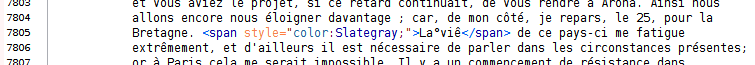
\includegraphics[width=16cm]{images/span_lamennais_7805.png}
    \label{span_lamennais_7805}
\end{figure}

Cependant, certaines fautes ne sont pas signalées par l'OCR, comme on peut le constater vingt lignes plus loin dans le même fichier.

\begin{figure}[ht]
    \centering
    \caption{Exemple d'une balise \citecode{<span>} manquante dans l'HTML du premier volume de Lamennais, l. 7825}
    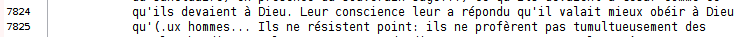
\includegraphics[width=16cm]{images/sans_span_lamennais.png}
    \label{sans_span_lamennais}
\end{figure}
Ici, le \inquote{a} est remplacé par une parenthèse ouvrante et un point. 

Enfin, parfois, les balises \citecode{<span>} sont présentes alors qu’aucune faute n’est à signaler, comme par exemple à la ligne 1264 où le guillemet est juste alors que signalé comme douteux, comme on peut le constater ci-dessous. 

\begin{figure}[ht]
    \centering
    \caption{Exemple d'une balise \citecode{<span>} superflue dans l'HTML du premier volume de Lamennais, l. 1264}
    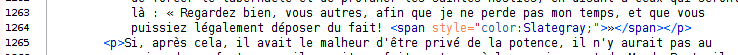
\includegraphics[width=16cm]{images/span_inutile_lamennais.png}
    \label{span_inutile_lamennais}
\end{figure}



\subsection{L'apport des expressions régulières dans le nettoyage de l'HTML}

L'idéal aurait été de toucher le moins possible à l'HTML et de ne faire que des traitements applicables à tous les autres volumes d'un même correspondant. 

Cependant, nous avons procédé tout de même à un nettoyage sommaire de l'HTML. Pour cela, les expressions régulières nous ont été un outil précieux. On entend par \inquote{expressions régulières} ou \inquote{regex}, de l'anglais \emph{regular expression}, une chaîne de caractères, qui décrit, selon une syntaxe précise, un ensemble de chaînes de caractères possibles. En l'utilisant dans un éditeur de texte, ou sinon dans Python, on peut ainsi \inquote{matcher}, c'est-à-dire sélectionner certaines suites de chaînes de caractères récurrentes et les sélectionner toutes ensemble, puis soit les remplacer par une autre chaîne de caractère, soit les supprimer définitivement. C'est donc très précieux pour faire des modifications dans les textes, et ici pour pré-traiter notre HTML.

Comme nous l'avons déjà évoqué plus haut, certains titres dans Lamartine polluaient le texte, comme on peut le constater dans la figure suivante~: tous les éléments inutiles y sont surlignés en jaune.

\begin{figure}[ht]
    \centering
    \caption{Exemple des titres polluant le texte, HTML de Lamartine}
    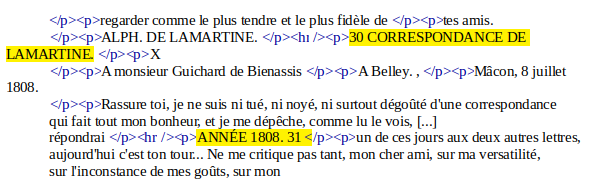
\includegraphics[width=16cm]{images/titres_lamartine.png}
    \label{titres_lamartine}
\end{figure}

Avec l'éditeur de texte Oxygen XML Editor, nous pouvons user des regex. C'est donc par ce biais que nous avons supprimé ces titres. 

\begin{figure}[ht]
    \centering
    \caption{Exemple d'une regex pour enlever certains titres, HTML de Lamartine}
    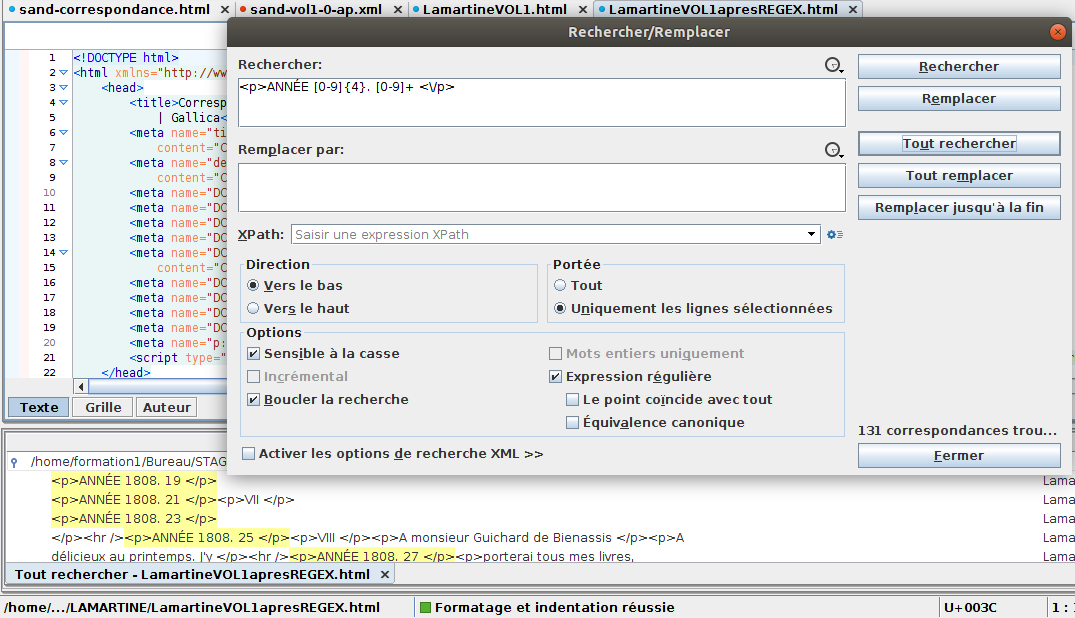
\includegraphics[width=16cm]{images/titres_annee_lamartine.png}
    \label{titres_annee_lamartine}
\end{figure}

La capture d'écran ci-dessus montre comment cela se présente~: on indique dans la fenêtre la regex, et en cliquant sur \inquote{tout rechercher}, 131 matches sont renseignés. Il suffit ensuite d'indiquer \inquote{tout remplacer} et l'HTML est donc nettoyé des 131 titres superflus. 

Malheureusement, nous ne pouvons trouver des regex applicables à tous les corpus étant donné qu'ils se présentent différemment. Ainsi, pour la correspondance de Proudhon, nous supprimons ces titres avec une regex qui diffère~: \citecode{<p>[0-9]\{1,3\} CORRESPONDANCE <\/p>}. Elle fait 108 matches.

De même, pour supprimer les \citecode{</p><p>} évoqués plus haut et coupant les phrases en deux, rompant ainsi l'unité, nous avons également utilisé les regex, cette fois-ci en indiquant que nous ne voulions supprimer que les \citecode{<p>} englobant des minuscules, car minuscules signifient phrases en cours.

\begin{figure}[ht]
    \centering
    \caption{Exemple d'une regex pour enlever des \citecode{<p>}, HTML de Lamartine}
    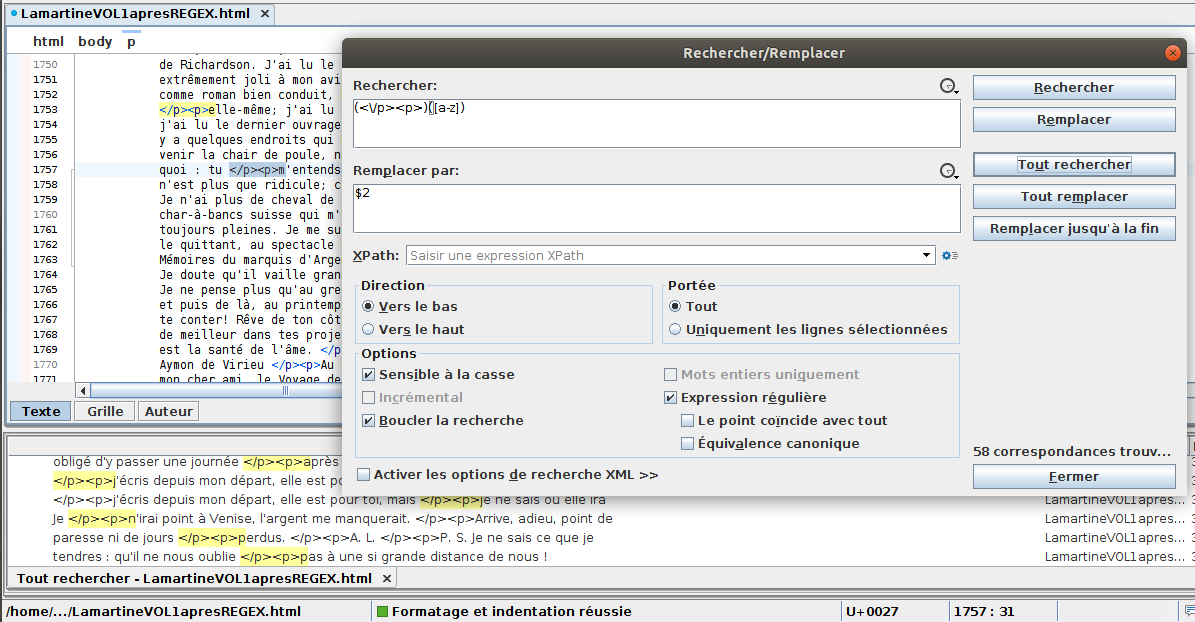
\includegraphics[width=16cm]{images/regex_p.png}
    \label{regex_p}
\end{figure}

Ici, nous matchons donc les deux balises \citecode{<p>} et nous mettons des parenthèses. Nous matchons celles qui se trouvent avant des minuscules (donc en milieu de phrase).
Pour la substitution, nous écrivons \citecode{\$2} comme cela les \citecode{<p>} sont supprimés et le \citecode{\$2} qui fait référence à la deuxième parenthèse garde le contenu et n’enlève pas la première lettre du mot en minuscules.

Ainsi, les expressions régulières permettent un gain de temps considérable dans le nettoyage de l'HTML.

\subsection{Quelle granularité dans la correction ?}

Cependant, celui-ci suscite des questionnements~: dans quel mesure faut-il corriger les fautes ? Quelle correction faire ? Une correction technique ou orthographique ? 

\subsubsection{Une correction orthographique ?}

Venant d'un parcours plus littéraire, il nous a été en effet très difficile de fermer les yeux sur certaines fautes, quitte à ce qu'elles soient corrigées par la suite. En effet, il nous a paru parfois plus judicieux de corriger en amont, c'est-à-dire dans l'HTML, certaines fautes orthographiques que nous avions remarquées, avant que celles-ci ne soient dispersées dans divers fichiers XML-TEI (en effet, la suite de la procédure est de diviser l'HTML en de multiples fichiers XML-TEI, un fichier par lettre)~: corriger les fautes en amont permettrait donc de pouvoir matcher les fautes dans un seul fichier HTML. Ainsi, nous nous sommes permis de faire quelques corrections orthographiques, dont nous donnons quelques exemples. 

Tout d'abord, un des problèmes de l’OCR est qu'il « recolle» un mot qui a été divisé par un tiret, lorsqu'il est en fin de ligne. 
Un problème se pose lorsque le mot en fin de ligne a un tiret parce que cela fait partie d’une expression, comme à la ligne 4026 de l'HTML de Lamartine où l’expression « écris-moi » a été assemblée en un mot « écrismoi\footnote{5 matches.} ». C'est donc une fausse interprétation de l'OCR qui ne fait pas la distinction entre un mot \inquote{recollé} avec raison ou non.Tombant dessus par hasard, nous avons donc corrigé ce genre d'erreurs. De même, l'OCR confond parfois les \inquote{l} et les \inquote{t}. Ainsi, quand nous sommes tombée sur ce genre d'erreurs, nous avons remplacé \inquote{Celte} par \inquote{Cette}\footnote{17 matches} ou \inquote{lu} par \inquote{tu}\footnote{70 matches, en faisant attention à ne pas corriger faussement certains \inquote{lu} qui sont justes (11 matches)}.

Ainsi, lorsque cela s'y prêtait, nous nous sommes permis de corriger certaines fautes qui s'imposaient à nous. Néanmoins, ce  n'était pas notre travail de les rechercher. Ce n'était pas notre objectif. Nous devions plutôt traquer les fautes techniques.

\subsubsection{Avant tout, une correction technique}

En effet, notre priorité était plutôt de corriger les balises comportant des problèmes, comme nous l'avons souligné plus haut (balises mal fermées, balises superflues, balises divisant des phrases en deux paragraphes). 

Parmi les fautes qui nous ont retenue figurait le manque de certaines balises pouvant poser problème par la suite pour l'extraction avec Python. En effet, cette extraction se base sur certains marqueurs. Si ceux-ci sont mélangés de temps en temps au reste du texte, les lettres ne sont pas bien extraites. Ainsi, pour ce qui est de la correspondance de Lamartine, il manquait des balises \citecode{<p>}  pour séparer la signature des chiffres romains désignant une nouvelle lettre~: \citecode{<p>ALPH. DE LAM. LXII</p>}. Nous les avons donc ajoutées avec une regex, pour les soixante-cinq occurences~: \citecode{<p>ALPH. DE LAM.</p><p>LXII</p>} 

En effet, il s'agit avant tout d'assurer une bonne extraction avec Python du fichier HTML pour qu'il soit transformé en fichiers XML. Pour cela, la dernière phase de pré-traitement est de repérer les marqueurs du texte en vue de l'extraction.


\subsection{Premiers repérages des marqueurs}

Les marqueurs avaient déjà été signalés dans le cahier de charges~: à chaque édition imprimée correspondent des caractéristiques différentes. Ainsi, pour la correspondance de Lamartine, on remarque que les lettres sont séparées les unes des autres par un chiffre romain. Celui-ci manquait parfois, nous nous sommes donc permis de l'ajouter manuellement, comme pour la deuxième lettre de Lamartine. Pour Lamennais, les lettres sont délimitées par des chiffres arabes cette fois. Ceux-ci posent problème car ils ne sont pas bien reconnus par l'OCR. Par conséquent, ils ne peuvent pas être extraits facilement avec des regex dans Python puisqu'ils comportent des erreurs~: le chiffre 5 est souvent pris pour un \inquote{a}, le 5 et le 3 sont souvent confondus, et le 8 est pris pour un \inquote{S}. Au lieu de 15, on lit \citecode{l.'l}, au lieu de 19, on lit \citecode{I!\&gt;}, à la place de 44, on trouve \citecode{t4}, et \citecode{ftj} pour 63, \citecode{tH} pour 64, pour n'en citer que quelques-uns. Nous avons donc dû retravailler ces marqueurs pour assurer une bonne extraction des lettres. Enfin, les lettres de Proudhon n'avaient pas de délimiteur. Nous nous sommes donc servie de sa signature \inquote{P.-J. PROUDHON.} pour extraire les lettres.

\begin{figure}[ht]
    \centering
    \caption{Cahier des charges ELICOM, repérage des marqueurs de Lamennais}
    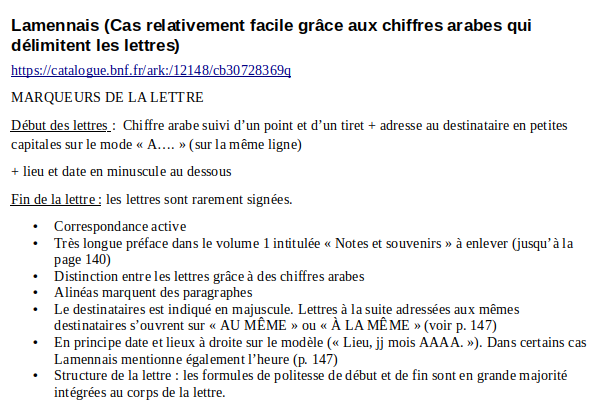
\includegraphics[width=16cm]{images/cdc_lamennais.png}
    \label{cdc_lamennais}
\end{figure}

Ainsi, l'OCR de Gallica s'est avéré être assez performant dans l'ensemble et nous a rendu de précieux services pour l'extraction de la correspondance en HTML. Bien-sûr, il reste quelques fautes à corriger, aussi bien au niveau de la structure de l'HTML qu'au niveau purement orthographique. Par ailleurs, nous n'avons pas encore évoqué la question de la mise en page qui n'est pas traitée par l'OCR, ce qui nous pénalise également. Nous y reviendrons lorsque nous parlerons des fichiers XML en quatrième partie. Néanmoins, le bilan est très positif pour l'OCR de Gallica. L'apprentissage machine a donc bien été au c\oe ur de l'acquisition des données pour notre projet d'ELICOM avec le Labex OBVIL. Il en est de même pour notre projet d'édition numérique de correspondance de Frédéric Le Play, même s'il se présente cette fois-ci sous la forme de l'HTR avec Transkribus.

\chapter{L'HTR de Transkribus}


\section{Quelle procédure pour l'acquisition des données ?}

\subsection{Rappels et point sur le corpus}

Il s'agit désormais d'acquérir les données pour notre projet d'édition numérique de la correspondance de Frédéric Le Play avec le CRHXIX. Avant tout, faisons un point sur le corpus en notre possession. Nous pensons pour l'instant éditer les  2091 lettres échangées entre Frédéric Le Play et 94 correspondants entre 1837 et 1882. 

En vue de leur mise en ligne, plusieurs étapes sont à suivre. Tout d’abord,avons-nous toutes les numérisations en notre possession, leur qualité est-elle suffisante ? De plus, les transcriptions ont-elles été réalisées ? Sinon, quelle procédure suivre pour réaliser ce travail ?

\subsection{S'assurer des numérisations des manuscrits}

Comme souligné plus haut, un travail de numérisation a déjà été engagé, et un récapitulatif a été fait sur les fonds numérisés\footnote{Voir fig. 3.1}. Il est en effet capital d'avoir une vue claire là-dessus car elles constituent la matière première, la base de notre travail. 

Plusieurs questions se posent sur la qualité de ces numérisations. En effet, comme nous l'avions déjà souligné dans notre deuxième partie\footnote{Voir 5.1.2},
\begin{quote}
    \inquote{Dans  le  cas  de la  publication  de  textes  en fac-similés [...],la  lisibilité  des  images  est  essentielle,  ce  qui  suppose  à  la  fois  une  attention  aux formats d’acquisition (qualité de l’image exprimée en dpi), et une juste évaluation des besoins de stockage et d’infrastructure matérielle pour la diffusion/communication de celles-ci\footnote{Ioana Galleron, Marie-Luce Demonet, Cécile Meynard, Idmhand Fatiha, Elena Pierazzo, etal., \emph{Les publications numériques de corpus d’auteurs - Guide de travail, grille d’analyse et recommandations}, 2018, URL~: \url{https://halshs.archives-ouvertes.fr/halshs-01932519/document}(visité le 05/05/2020).}}
\end{quote}
Or, si nombre de numérisations sont satisfaisantes car elles ont été commandées à des services d'archives ou bibliothèques, pour d'autres manuscrits, nous ne possédons que des photographies prises par des particuliers et qui sont floues ou d'une qualité médiocre, tant pour la précision que pour la prise de vue. Il s'agira donc de les faire numériser par des professionnels.

Par ailleurs, nous nous posons encore la question du format de l'image. Serait-il bon d'unifier les formats ? Nous avons tantôt des fac-similés en JPEG, tantôt des PDF ou encore TIFF (\emph{Tagged Image File Format}), plus rarement des PGN (\emph{Portable Network Graphics}). Il serait bon d'unifier les formats mais nous ne pensons pas que cela soit indispensable\footnote{Le retour en arrière aurait un coût probablement trop important alors que non indispensable}. L'important surtout est d'obtenir un fichier par page. C'est là que nous avons rencontré des problèmes avec certains PDF trop lourds, notamment ceux de la BNF et de la BIF, car ils comprenaient un trop grand nombre de pages~: il faudrait donc diviser les fichiers pour qu'il y ait un seul fichier par page numérisée\footnote{Par page numérisée, et non par lettre qui comprend parfois plusieurs pages}, que l'on pourrait ensuite appeler dans le fichier XML-TEI comprenant la transcription correspondante.

En vue de l’édition numérique de correspondance, il serait bon de privilégier les numérisations en couleur pour le design du site. La majorité, si ce n’est l’intégralité des sites d’édition numérique de correspondance possèdent des numérisations en couleur. Le but de mettre en ligne le manuscrit est de coller au plus près de la réalité matérielle.Dans ce but, la numérisation en couleur est préférable. Certes, nous possédons, notamment pour les fonds Peruzzi et Loyson, des numérisations en noir et blanc, qui sont d’ailleurs de très bonnes qualité. On pourrait à long terme songer à les remplacer par des numérisations en couleur, mais cela ne nous semble pas du tout prioritaire. Le site de Flaubert que nous avons déjà évoqué ne met pas toujours en ligne des fac-similés en regard, et certains sont en couleur, d'autres en noir et blanc. Certes, ce n'est pas parfait mais cela n'enlève rien à la qualité du site.

Par ailleurs, il faudra être attentif au nommage de chaque fichier, procédant toujours de la même manière, comme par exemple \citecode{expediteur\_destinataire\_fonds\_lettre1a.jpg}, en abrégeant les noms selon ce qui a été fixé. Ainsi, on pourrait écrire \citecode{lp\_ribbe\_arbaud\_l1b.jpg} ce qui signifie~: lettre de Frédéric Le Play à Charles de Ribbe, musée Arbaud, lettre 1, page 2 (pour le b)\footnote{Cette proposition reste encore un peu longue. On pourrait trouver quelque chose d'aussi précis mais de plus court.}.


Ainsi, avant tout, il s'agit de s'assurer de la bonne qualité des fac-similés et de leur bon nommage.
Ceci fait, on peut commencer à transcrire, puisque nous ne voulons pas seulement éditer les fac-similés. Nous voulons aussi avoir leur transcription en regard. Comment y parvenir pour ce corpus si important ? N'y aurait-il pas possibilité d'automatiser tout cela pour aller plus vite ?

\subsection{Transcriptions manuelles ou automatisées ?}
	
Nombre de manuscrits\footnote{Quelques centaines probablement, nous n'avons pas le chiffre exact.} ont déjà été transcrits manuellement, comme souligné plus haut, que cela soit par des étudiants, des doctorants, des stagiaires.
Or, la transcription s’avère être parfois un exercice difficile : les hommes du XIX\up{e} siècle disposent de certains codes d’écriture ou d’abréviations\footnote{Comme par exemple pour la date qui est souvent chiffrée différemment. Ainsi, ils écrivent 7bre pour septembre, Xbre pour décembre etc.} qui ne nous sont pas familiers. Par ailleurs, nombre de mots sont difficiles à lire, du fait des différentes écritures. Je pense par exemple à celle de Jules Baroche\footnote{Voir Annexe B.1 issue des premières pages du PDF SIM MS 6062 (p.7). Jules Baroche par exemple, lorsque deux « s » se suivent, allonge le premier. Ce sont les \inquote{s} longs que nous évoquions plus haut}.
Même avec un œil exercé, et des mains habituées à taper rapidement, il faut compter au moins cinq minutes par page pour la transcription, sans compter la relecture. En une heure, on peut donc transcrire douze pages, sans compter la relecture, ce qui nécessite deux-cents heures de transcription pour deux-mille lettres.

Ainsi, sur un corpus aussi important, comportant plus de deux-mille lettres, la question se pose d’automatiser les transcriptions en utilisant les moyens technologiques dont nous disposons aujourd’hui notamment avec l’apprentissage machine. C’est ainsi que nous avons fait le choix de nous tourner vers Transkribus.


\section{Transkribus, un outil de transcription}

\subsection{Transkribus, un pari}

Transkribus est un outil utilisé par de nombreux projets, mais il n’est pas forcément approprié à tous les corpus. Une transcription « manuelle » nécessite, certes, beaucoup de temps et une relecture attentive, mais entraîner une machine telle que Transkribus nécessite également beaucoup de temps, et ceci avec l’incertitude du résultat. 
S’il y a plus de 90 \% de taux de réussite, la transcription pourra se faire sans trop de difficultés, mais la relecture restera longue et nécessaire. S’il y a 98 \% de taux de réussite, c’est à nous de voir si nous acceptons ce taux d’erreurs ou si nous préférons relire pour un rendu plus optimal, mais également plus coûteux en temps, sachant que nous aurons de toutes façons les fac-similés en regard.

Par ailleurs, comme le soulignent les tutoriels mis en ligne pour initier à Transkribus, il faut \inquote{du temps pour explorer Transkribus et se familiariser avec son fonctionnement\footnote{Régis Schlagdenhauffen, \emph{Comment utiliser Transkribus en 10 étapes (voire moins)}, Site web de l'EHESS, URL~: \url{http://regis-schlagdenhauffen.eu/wp-content/uploads/2018/01/Comment-utiliser-Transkribus-\%E2\%80\%93-en-10-\%C3\%A9tapes-ou-moins.pdf} (visité le 22/05/2020).)}}. C’est donc un réel investissement au début, avec l’incertitude du résultat et la possibilité d’un échec.

Pour notre part, les résultats ont été dès le début encourageants. Sur 16 lettres, nous avons obtenu des scores de 84~\% d'erreur sur les caractères en entraînement. 
Nous avons donc continué cette aventure virtuelle, encouragés que nous étions par ces premiers retours.
Avant de présenter plus en détail notre travail sur Transkribus, il importe de présenter plus en détail cet outil.

\subsection{Un outil pensé par le READ}

\subsubsection{Le projet}

L' EADH, association européenne pour les humanités numériques (en anglais \emph{European association for digital humanities}), fondée en 1973\footnote{Sous le nom de \emph{Association for Literary and Linguistic Computing} (ALLC), voir \emph{About}, Site web de l'EADH, URL~: \url{https://eadh.org/about}, (visité le 23/09/2020).}, rassemble en son sein de nombreux projets pour faire avancer les humanités numériques\footnote{Le projet \emph{correspSearch} évoqué dans la deuxième partie en fait partie.}. Parmi eux, le projet READ\footnote{Projet lancé en 2015}, \emph{Recognition and Enrichment of Archival Documents} tient une place toute particulière. Comme son nom l'indique, il se consacre à la reconnaissance et à l'enrichissement des documents d'archives, visant à rendre les documents d'archives plus accessibles grâce à l'utilisation de technologies de pointe. L'objectif principal de READ est de fournir une plate-forme de services\footnote{Voir \emph{Accueil, Site web de Transkribus, URL~: }\url{http://transkribus.eu} (visité le 06/03/2020).} pour la reconnaissance, la transcription et la recherche automatisées de documents historiques. Entraîner les ordinateurs à lire du texte manuscrit de cette manière promet de révolutionner l'accès aux archives écrites. C'est dans cette optique que l'outil de transcription Transkribus a été conçu.

\subsubsection{L'outil}

Transkribus est un logiciel de transcription collaborative. 
Pour l'utiliser, il suffit de s'inscrire et de le télécharger. Puis, on peut importer les manuscrits en n'importe quelle langue, les transcrire manuellement, seul ou en équipe, en liant le texte à l'image grâce à la segmentation des images en régions de textes, lignes et mots réalisée à l'aide d'outils d'analyse de disposition. Puis avec ces transcriptions, on peut entraîner un modèle qui permettra à Transkribus de reconnaître par la suite l’écriture en question et d’effectuer lui-même les transcriptions.	

\subsection{Transkribus et l'apprentissage machine}

Transkribus s'utilise aussi bien pour l'OCR que pour l'HTR, mais ceux-ci diffèrent. En effet, 
\begin{quote}
    \inquote{La reconnaissance du texte manuscrit est un champ à part entière au sein des systèmes d’OCR. On parle d’ailleurs de \emph{Handwritten text recognition} (HTR) pour désigner le traitement des documents manuscrits, preuve qu’ils nécessitent des technologies spécifiques\footnote{\emph{in} Alix Chagué, \emph{ibidem.} p.42.}.}
\end{quote}
L'HTR n'est pas comme l'OCR, où, comme on a pu le remarquer avec l'OCR de Gallica, on appuie sur le bouton et le document est reconnu automatiquement. Qui dit HTR dit entraînement adapté à l'écriture d'une main particulière, sachant que cette main peut varier d'écriture ce qui rend l'entraînement d'autant plus fastidieux. Ainsi, Transkribus se doit d'entraîner des modèles\footnote{\emph{Handwritten Text Recognition Workflow}, Wiki de Transkribus, URL~: \url{https://transkribus.eu/wiki/index.php/Handwritten_Text_Recognition_Workflow} (visité le 23/09/2020).}. Pour cela, il est nécessaire de transcrire préalablement 100 pages, soit 15 000 à 20 000 caractères. 

En réalisant ce travail, nous participons de près ou de loin à l'objectif du READ. En effet, le but à long terme est d'entraîner le plus de styles d'écriture différents, de manière à ce que Transkribus soit en mesure de traiter la plupart des documents manuscrits sans entraînement préalable. Plus les utilisateurs travailleront avec Transkribus pour leur transcription, plus vite cet objectif ambitieux sera atteint\footnote{\emph{Questions and Answers}, Wiki de Transkribus, URL~: \url{https://transkribus.eu/wiki/index.php/Questions_and_Answers} (visité le 23/09/2020)..}. 

\subsection{Point sur la terminologie}

Avant de voir comment nous avons procédé avec Transkribus, il est utile de faire un point sur la terminologie en usage dans l'apprentissage machine\footnote{Voir \emph{ML | Introduction to Data in Machine Learning}, Site web GeeksforGeeks, URL~: \url{https://www.geeksforgeeks.org/ml-introduction-data-machine-learning/} (visité le 02/06/2020).. La figure 9.1 est tirée de cet article.}. Par ailleurs, l'anglais étant la norme en informatique, comment rendre les termes en français ? 

\begin{figure}[ht]
    \centering
    \caption{Les données dans l'apprentissage machine}
    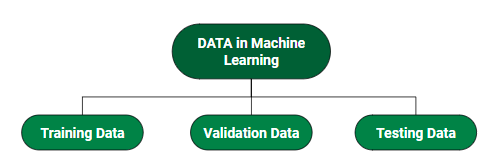
\includegraphics[width=16cm]{images/terminologieML.png}
    \label{terminologieML}
\end{figure}

Les données dans l'apprentissage machine se divisent en trois catégories, comme nous pouvons le voir sur la figure ci-dessus\footnote{Pour nous, les données en général sont les manuscrits. Mais en soi, les données peuvent être du texte, des sons et images etc.~: \inquote{\emph{It can be any unprocessed fact, value, text, sound or picture that is not being interpreted and analyzed}} \emph{In ibidem.}}~: 
\begin{itemize}
    \item Les données d'entraînement ou \emph{Training Data}~: ce sont les données que nous utilisons pour entraîner le modèle et qu'il apprend.
    
    Dans Transkribus, on appellera ces données \emph{Training Set}\footnote{Voir \emph{How to transcribe. Train a model}, Wiki de Transkribus, URL~: \url{https://transkribus.eu/wiki/images/3/34/HowToTranscribe_Train_A_Model.pdf} (visité le 23/09/2020), traduit en français~: \emph{Entraînement d’un modèle dans Transkribus}, Wiki de Transkribus, URL~: \url{https://transkribus.eu/wiki/images/8/84/Comment_entra\%C3\%AEner_un_Mod\%C3\%A8le_dans_Transkribus.pdf} (visité le 22/05/2020).} ou set d'entraînement\footnote{\emph{Entraînement d’un modèle dans Transkribus}, Wiki de Transkribus, URL~: \url{https://transkribus.eu/wiki/images/8/84/Comment_entra\%C3\%AEner_un_Mod\%C3\%A8le_dans_Transkribus.pdf} (visité le 22/05/2020).}. 
    
    \item Les données de validation ou \emph{Validation Data}~: elles sont utilisées pour évaluer le modèle d'après les données d'entraînement.
    
    \item Les données de test ou \emph{Testing Data}~: elles permettent d'évaluer la qualité du modèle une fois qu'il est entraîné. Le modèle prédit le taux d'erreur à chaque fois avec les données de test. D'une fois à l'autre, nous pouvons ainsi voir la progression du modèle par l'expérience. En effet, plus nous rentrons de données d'entraînement, plus le modèle acquiert de l'expérience, moins il se trompe, plus le taux de réussite est important et donc le taux d'erreur moindre.
    
    Pour Transkribus, pendant le processus de formation, quelques pages sont mises de côté à titre de test. Elles ne sont pas utilisées pour l'entraînement du modèle HTR+. Elles sont plutôt utilisées pour tester les performances de notre modèle\footnote{\emph{Idem.}, p.7}.
\end{itemize}

Ainsi, la plate-forme Transkribus permet aux utilisateurs d‘entraîner un modèle HTR+ de reconnaissance automatique de documents. Le modèle doit être entraîné pour reconnaître un style d'écriture particulier. Cela se fait en lui "montrant" les images et les transcriptions exactes correspondantes\footnote{\emph{Ibid.}, p.3}.

Voyons plus en détail comment procéder à l'acquisition des données pour notre projet avec l'outil de transcription Transkribus.

\section{Chargement des données d'entraînement et premier traitement}

\subsection{Procédure pour le chargement des données d'entraînement}

Pour charger les données d'entraînement, il y a toute une procédure à suivre. Il s'agit d'indiquer à la machine à quoi correspond tel caractère pour l'aider à apprendre l'écriture de Frédéric Le Play afin de pouvoir par la suite procéder elle-même aux transcriptions. 

Après avoir importé les données, on divise le texte en \emph{Text Region} (TR) ou régions de texte~: on lui indique où se trouve l'écriture. Puis on la lance pour que, dans ce cadre donné, elle tente de reconnaître elle-même où sont les lignes et surtout les \emph{base line} (BL), c'est-à-dire le trait à la base d'une ligne. En général, la Transkribus fait bien le travail, mais parfois, dès cette étape, on est en bute à certains dysfonctionnements lorsque la page comprend deux sens d'écriture.  

\begin{figure}[H]
    \caption{Résolution du problème de TR, deux sens d'écriture, capture d'écran de Transkribus}
    \centering
    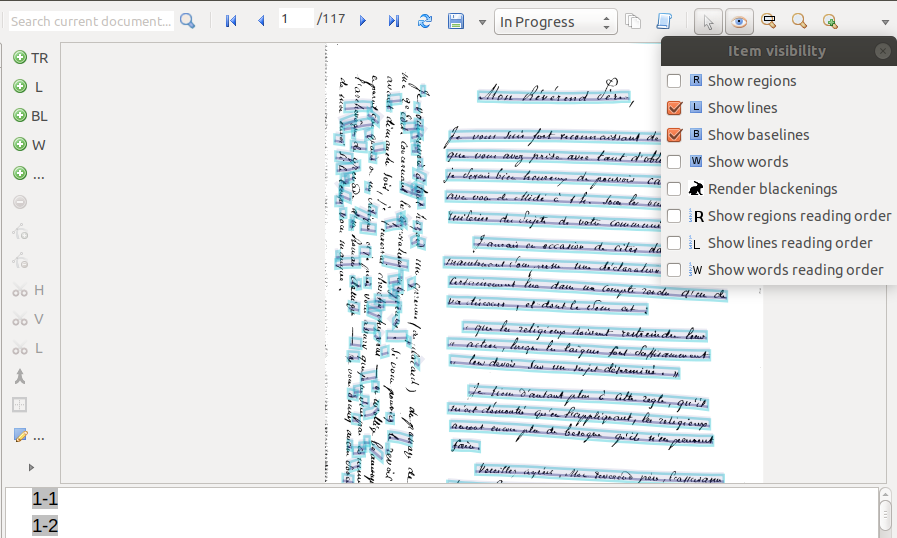
\includegraphics[width=7.5cm]{images/trTranskribus.png}
    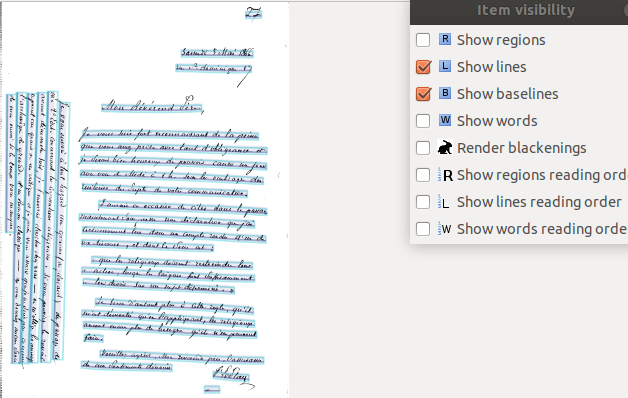
\includegraphics[width=7.5cm]{images/trCorrTranskribus.png}
\end{figure}

Transkribus se trompe alors totalement et reconnaît à la fois une multitude de lignes et de TR\footnote{Voir fig. 9.2}~: on peut gagner du temps en supprimant par TR (cela supprime du même coup les lignes que la TR a en son sein) mais quand il y a de multiples TR, on est obligé de tout supprimer à la main ce qui est une première perte de temps\footnote{Voir la version agrandie de ces deux images dans les annexes B.2}.\\

De même, quand Le Play utilise un papier légèrement strié pour écrire, celui-ci est confondu avec les caractères et considéré comme des lignes d'écriture\footnote{Voir fig. 9.3}. Il signale donc des lignes qui n'en sont pas. Ici, le mieux est de supprimer la TR et de mettre les BL manuellement, de gauche à droite et non l'inverse, sinon, la ligne apparaît en-dessous de la BL.\\

\begin{figure}[ht]
    \centering
    \caption{Problème de TR à cause du papier, capture d'écran de Transkribus}
    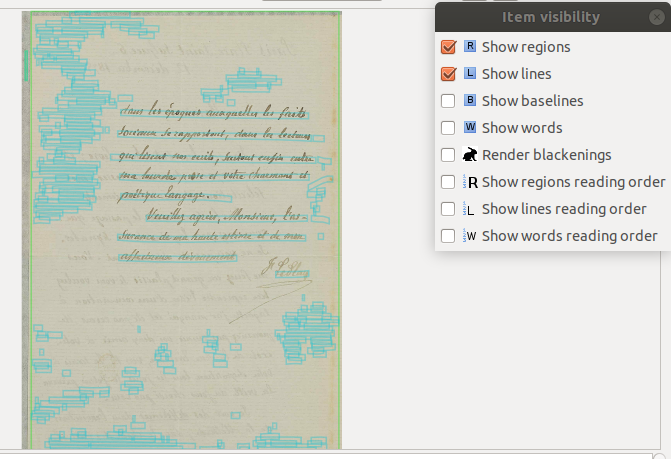
\includegraphics[width=13cm]{images/strieTranskribus.png}
    \label{strieTranskribus}
\end{figure}


Puis on peut procéder à la copie des transcriptions. Pour cela, on procède par copier/coller si les transcriptions ont déjà été réalisées, ce qui est notre cas. 
Néanmoins, cette phase nécessite une attention particulière. En effet, la mise en page et certaines graphies, lorsque l'on copie/colle, ne sont pas prises en compte. Il s'agit donc de les renseigner au fur et à mesure dans Transkribus. 

Transkribus permet ainsi d'indiquer les exposants, les mots qui ne sont pas clairs ou illisibles (\emph{unclear}), les mots barrés (\emph{strikethrough}), les mots soulignés(\emph{underlined}) etc.\footnote{Voir annexe B.3, fig. B.6, les styles de transcription en jaune.}..

Or, cette phase de chargement des données d'entraînement suscite d'autres questionnements sur les transcriptions. 


\subsection{Des transcriptions qui suscitent des questionnements}

\subsubsection{Des transcriptions de qualité variable}

Avant tout, nous avons commencé par importer les manuscrits dans Transkribus. Pour cela, il faut savoir lesquels nous désirons traiter en priorité. Notre choix s'est arrêté sur l'écriture qui ressort majoritairement du corpus en notre possession, à savoir celle de Frédéric Le Play. Ceci posé, nous avons commencé par importer dans Transkribus les manuscrits, puis les transcriptions qui avaient déjà été réalisées pour le CRHXIX. Nous avons dressé un tableau pour classer les correspondances à traiter en premier, en commençant par celles qui étaient de meilleure qualité quant à la numérisation et à la transcription, pour finir avec celles qui étaient de moindre qualité. En effet, certaines transcriptions ont déjà été relues ce qui est une garantie de meilleure qualité.

D'autres transcriptions faites par des étudiants n'ont pas encore été relues, par manque de temps, comportant des erreurs souvent dues à un manque compréhensible de familiarité avec les documents du XIX\up{e} siècle. Par ailleurs, certaines corrections notamment dans les accentuations ont été faites dans les transcriptions. Comment gérer ces différences par rapport aux originaux, alors que nous voulons justement charger des données pour apprendre à la machine à reconnaître les caractères ?

\subsubsection{Difficultés de transcriptions}

En une dizaine de jours, nous avons été amenée à rentrer 20 000 caractères dans le serveur de Transkribus afin d'entraîner le modèle pour l'écriture de Frédéric Le Play. 

De notre côté, nous n'avons pas fait de transcriptions à proprement parler, mais nous avons dû copier/coller les transcriptions réalisés par les étudiants et stagiaires pour le CRHXIX. Or, nous avons eu quelques doutes lors de la manipulation de ces transcriptions~: celles-ci n'étant pas toujours exemptes de fautes, nous nous sommes demandée dans quelle mesure nous devions les corriger.

Plusieurs questions émergent.

Tout d'abord, d'un point de vue purement technique, comment la machine peut-elle apprendre des caractères que nous-mêmes peinons à distinguer ? Ainsi, le \inquote{z} de Le Play est parfois écrasé et ressemble fort à un \inquote{r}~: cela a nécessité de notre part une certaine attention pour vérifier l'orthographe parfois incertaine des transcriptions d'une part, et d'autre part nous nous sommes demandée si la relecture des transcriptions opérées par Transkribus ne demanderait pas beaucoup de travail étant donné que les caractères sont souvent mal formés et donc difficiles à lire, et par l'\oe il humain, et par la machine, c'est du moins ce que nous craignons\footnote{Il est possible que par la suite, Transkribus sache mieux lire que l'homme, mais vu l'avancement du modèle de Le Play aujourd'hui, malgré les 20 000 caractères rentrés pour l'entraînement, ce n'est pas le cas.}. On constate ci-dessous que le \inquote{z} de \inquote{connaissez} pourrait être pris pour un \inquote{r}.

\begin{figure}[ht]
    \centering
    \caption{F. Le Play au R. P. Hyacinthe Loyson, 1866, capture d'écran de Transkribus}
    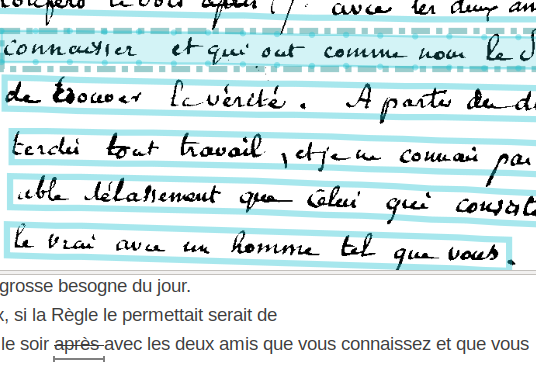
\includegraphics[width=12cm]{images/r-zTranskribus.png}
    \label{r-zTranskribus}
\end{figure}

Par ailleurs, nous avons dû être attentives à certaines mauvaises interprétations, comme par exemple, on lit dans la transcription~: \inquote{Que de bien à faire par le bon exemple ! car les sermons de vertu déposées [sic] pendant le moyen-âge ont percuté çà et là chez les vieillards. }

\begin{figure}[ht]
    \centering
    \caption{F. Le Play au R. P. Hyacinthe Loyson, 1866, capture d'écran de Transkribus}
    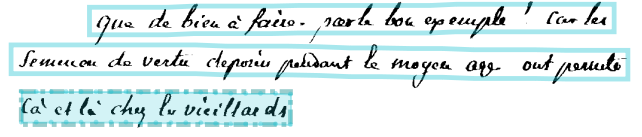
\includegraphics[width=16cm]{images/ma-Transkribus.png}
    \label{ma-Transkribus}
\end{figure}
Alors qu'il faudrait lire ce nous semble~: \inquote{Que de bien à faire par le bon exemple ! car les 
semences de vertu  déposées pendant le moyen âge ont persisté
çà et là chez les vieillards.}

Néanmoins, ces premières transcriptions même non relues sont d'une aide extrêmement précieuse~: le fait d’avoir déjà une grille de lecture aide à se mettre dans l’esprit du texte et à mieux saisir les possibles erreurs. C’est plus facile que si on aborde les textes avec un esprit totalement neuf. En outre, on peut bien dire qu'une des vertus de Transkribus est de nous permettre de réviser certaines transcriptions\footnote{À ce sujet, voir dans les livrables du CRHXIX le dossier \citecode{3-transcriptions} et l'explication dans les annexes.} 

On remarque ici par ailleurs la cédille manquante au mot \inquote{çà}, et l'accent circonflexe manquant sur le \inquote{a} de \inquote{âge} dans le manuscrit original. Par ailleurs, l'espace entre la préposition \inquote{par} et l'article défini \inquote{le} et si restreint qu'on croirait lire au premier regard \inquote{parle}. En trois lignes, on voit donc les complexités de transcriptions posées par l'écriture de Le Play.\\

Cette complexité se retrouve également face à certains mots difficilement lisibles et signalés comme illisibles par les premiers transcripteurs. Nous-même avons parfois peiné à saisir le sens de certains mots. Avec l'aide de l'équipe, nous avons pu venir à bout de certaines difficultés, comme ci-dessous\footnote{Fig. 9.6} où la graphie doublée des bavures de l'encre nous ont fait buter sur certains mots.  

\begin{figure}[ht]
    \centering
    \caption{F. Le Play au R. P. Hyacinthe Loyson, 1867, capture d'écran de Transkribus}
    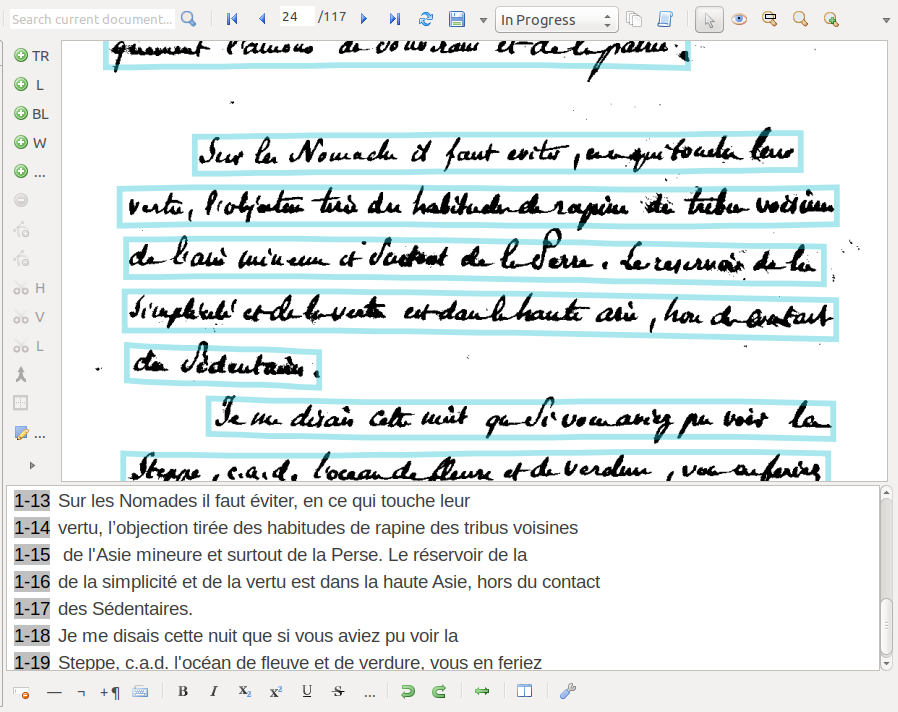
\includegraphics[width=16cm]{images/asieTranskribus.png}
    \label{asieTranskribus}
\end{figure}

\subsubsection{Transcriptions et principes de transcription}

Une des plus grandes difficultés pour nous a été aussi de faire la part des choses entre les majuscules justifiées ou non. Dans les principes de transcription évoqués plus haut\footnote{Voir 5.2.3.1}, il avait été convenu de respecter l’usage des majuscules par Le Play lorsqu’il semble avoir un sens précis, selon ses usages. Par exemple, Réforme plutôt que réforme ; ou les Autorités Sociales et de retenir l’usage
actuel lorsque les majuscules n’ont pas lieu d’être~: par exemple, \inquote{le concours de nos amis}, et non pas \inquote{le Concours de nos Amis}.
Cependant, certains cas particuliers nous ont laissée (peut-être à tort) perplexe. En effet, on remarque parfois une logique dans les majuscules chez Le Play. Faut-il la conserver ? Ici, Le Play écrit	\inquote{Vous remarquerez que dans mon Nouveau Plan, les anciens \underline{Chapitres}\footnote{Nous soulignons ici au lieu de mettre en italiques car nous reproduisons ce qui apparaîtra sur le site. Les mots soulignés et barrés apparaîtrons ainsi.}  deviennent des \underline{Livres} ; et que les anciens \underline{Paragraphes} deviennent des Chapitres.} 

\begin{figure}[ht]
    \centering
    \caption{F. Le Play au R. P. Hyacinthe Loyson, 1866, capture d'écran du manuscrit}
    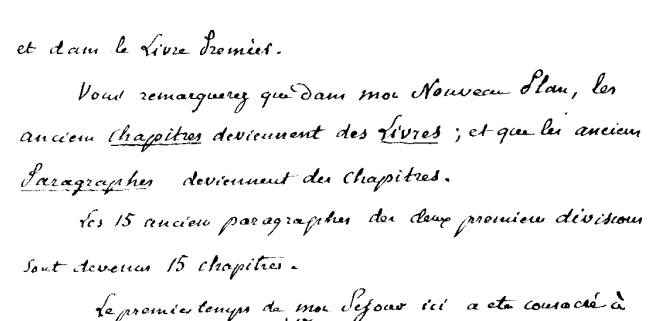
\includegraphics[width=16cm]{images/majusculesTranskribus.png}
    \label{majusculesTranskribus}
\end{figure}

En réalité, Le Play met des majuscules quand il veut insister sur un mot, qu'il souligne en plus de mettre une majuscule. Une fois que c’est établi, il continue sans majuscules :
\inquote{Les 15 anciens paragraphes des deux premières divisions sont devenus 15 chapitres}. Dans ce cas-là, pour notre part, nous serions pour conserver l'esprit de l'auteur de ces lettres en conservant la forme, et donc laisser les majuscules. Quant aux mots \inquote{Livre Premier} et \inquote{Nouveau Plan}, ils répondent également à la logique d'insistance de Le Play donc nous serions pour garder les majuscules. Néanmoins, nous enlèverions la majuscule à \inquote{Sejour} et ajouterions un accent aigu sur le \inquote{e} car c'est un autre cas de figure. La frontière est donc parfois difficile à voir entre la conservation ou non des majuscules.\\

\subsubsection{Des transcriptions qui ont pour but d'entraîner un modèle}

Une remarque s'impose~: nous rentrons ici des données d'entraînement en vue de la création d'un modèle qui permettra de transcrire automatiquement les lettres de Le Play. Si nous souhaitons que le modèle soit bien entraîné, il faut rentrer les données de façon brute, sans tri (majuscule ou non ? accent ou non ?). Ces questions ne devront se poser qu'au moment des relectures de transcription, après le travail de transcription sur Transkribus. Pour l'instant, nous devons respecter l'écriture de Le Play telle qu'elle apparaît sur le manuscrit, et non enlever des majuscules, ajouter des accents.\\

En revanche, c'est le moment où il s'agit de déchiffrer les mots classés illisibles par les premiers transcripteurs et corriger les fautes de transcription, ce que nous avons déjà évoqué plus haut.

Ici malheureusement, nous avons dû peu à peu lâcher du lest et baisser nos exigences. Comment pouvions-nous en si peu de temps coller entièrement au texte et corriger les premières transcriptions ? Rentrer 20 000 caractères n'est pas une mince affaire et représente une centaine de pages environ~: à la fin, nous avons été contrainte de nous contenter à faire des copiés/collés et corriger simplement les fautes qui sautaient aux yeux.\\

Une fois les caractères rentrés, il s'agit de procéder à l'entraînement du modèle, au fur et à mesure~: on peut constater ainsi la progression de l'apprentissage machine.

\section{Entraînement d'un modèle. Quels résultats ?}

\subsection{Mise en place de l'entraînement}

Peu à peu, on commence à entraîner le modèle. Plus on a de données d'entraînement, plus le modèle se perfectionne. 

On sélectionne les pages de transcription et on les met dans le \emph{Training Set}, puis on met de côté 10~\% des données dans le \emph{Validation Set} qui compare ce que nous avons transcris avec ce que la machine reconnaît après avoir été entraînée\footnote{Voir la figure 9.8 où on peut observer la sélection entre \emph{Training Set} et \emph{Validation Set}, juste avant de cliquer sur \inquote{OK} pour lancer l'entraînement du modèle. Ici, nous n'avions mis qu'une page pour le set de validation ce qui était normal car nous n'avions pas encore beaucoup de données et une page représentait donc environ 10~\%.}. 
\begin{figure}[ht]
    \centering
    \caption{Mise en place du premier entraînement du modèle Le Play}
    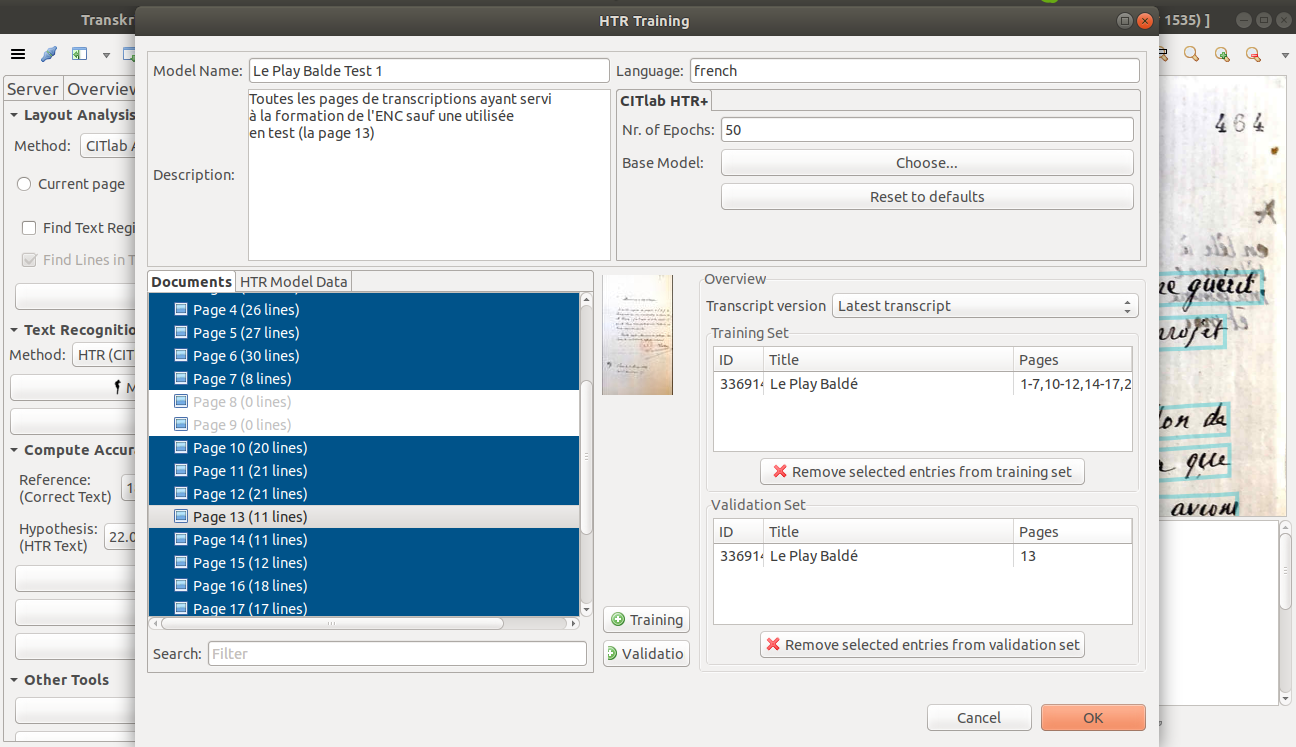
\includegraphics[width=16cm]{images/HTRtraining.png}
    \label{HTRtraining}
\end{figure}
Il est conseillé de prendre à chaque fois le même set de validation pour se faire une meilleure idée des progrès réalisés par l’apprentissage de la machine. De ce point de vue, notre entraînement du modèle a péché car nous n'avons pas mis assez de données de côté pour le set de validation. Nous pensions qu'il ne fallait mettre qu'une page alors qu'il fallait mettre 10~\%. Nous avons donc rectifié pour les derniers entraînements, mais cela fausse donc un peu la courbe de progression.\\

\subsection{Quelle progression du modèle, quels résultats ?}

Celle-ci est annoncée à la fin de chaque nouvel entraînement. On parle alors de \emph{Learning Curve} ou courbe d'apprentissage. On voit donc ci-dessous\footnote{Cf. Fig. 9.9} le graphique de la courbe d'apprentissage du premier entraînement du modèle Le Play. À gauche figurent tous les modèles disponibles, et tout en haut, en grisé, la ligne qui sélectionne le modèle qui nous intéresse et qui apparaît dans la colonne de droite.

\begin{figure}[ht]
    \centering
    \caption{\emph{Learning Curve} du premier entraînement du modèle Le Play}
    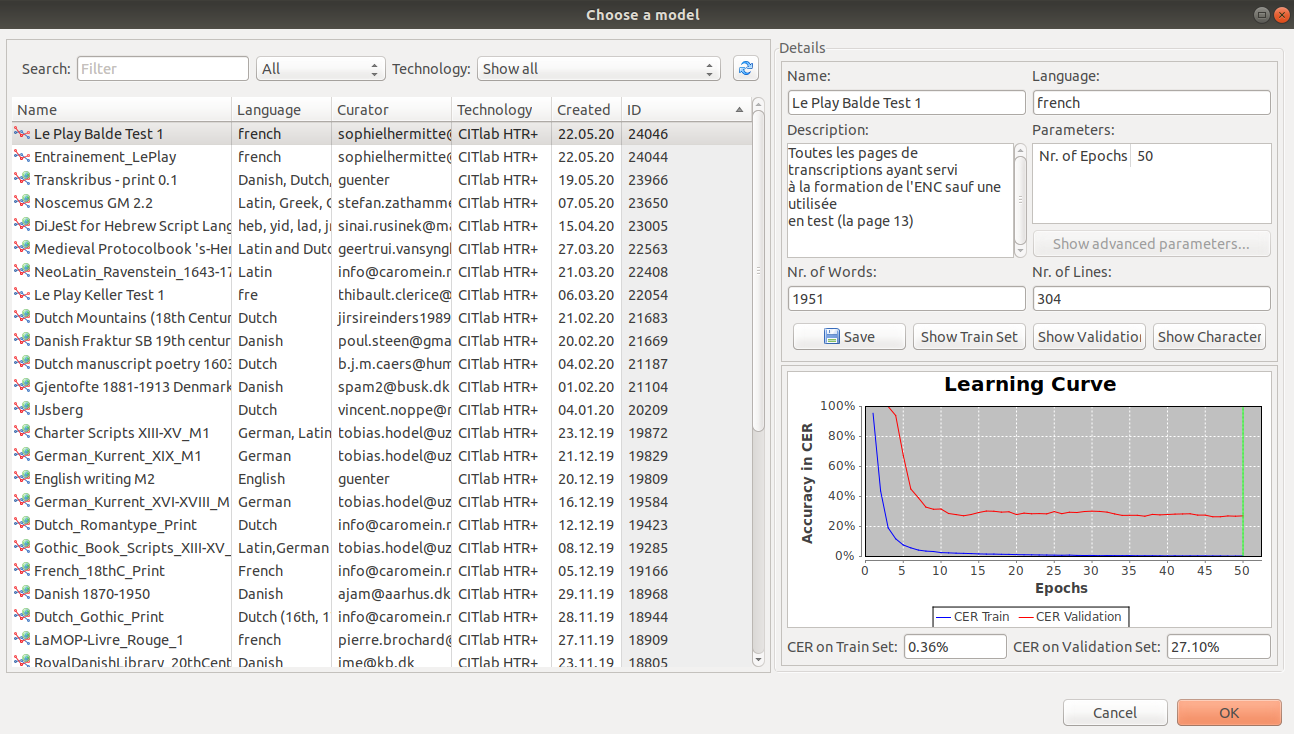
\includegraphics[width=16cm]{images/learningCurve.png}
    \label{learningCurve}
\end{figure}

Le taux d'erreurs de reconnaissance de caractères ou \emph{Character Error} (CER) définit l'efficacité du modèle. Cela représente le taux (en~\%) de caractères qui n'ont pas été
correctement transcrits par l‘HTR. L'idéal serait d'atteindre un CER inférieur à 5~\%, même si en soi un taux CER inférieur à 10~\% est déjà un taux satisfaisant.

Voyons plus en précision le graphique de la courbe d'apprentissage qui illustre la précision du dernier modèle entraîné\footnote{Cf. Fig. 9.10}, avec des données d'entraînement riches de 3146 lignes soit 23 729 mots.
 
 \begin{figure}[ht]
    \centering
    \caption{\emph{Learning Curve} du dernier entraînement du modèle Le Play}
    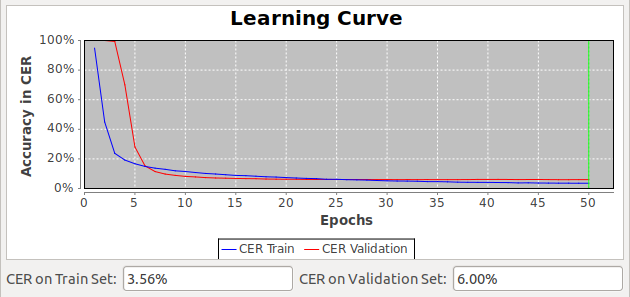
\includegraphics[width=16cm]{images/LearningCurveV4.png}
    \label{LearningCurveV4}
\end{figure}
 
Comme précisé dans le tutoriel fourni par Transkribus\footnote{\emph{Entraînement d’un modèle dans Transkribus}, Wiki de Transkribus, URL~: \url{https://transkribus.eu/wiki/images/8/84/Comment_entra\%C3\%AEner_un_Mod\%C3\%A8le_dans_Transkribus.pdf} (visité le 22/05/2020).}, l'axe Y définit l'\emph{Accuracy in CER} soit la précision en CER qui est affichée en pourcentage sur l'axe des ordonnées. La courbe
commence toujours à 100~\% et descend au fur et à mesure que l'entraînement progresse et que le modèle s'améliore.

L'axe X est défini comme \emph{Epochs} soit époques. Pendant le processus de formation, Transkribus effectue une évaluation après chaque époque. Lorsqu'on entraîne un modèle, on spécifie le nombre d'époques dans lesquelles le \emph{Training set} doit être divisé. Plus il y a d'époques, plus la formation dure longtemps. Ici nous en avons choisi 50.

Deux lignes apparaissent sur le graphique : une rouge qui indique l'état d'avancement des évaluations dans le jeu de tests et une bleue qui indique la progression de l'entraînement. \inquote{Le programme s'entraîne d'abord dans le \emph{Training Set}, puis se teste à l'aide des pages du \emph{Validation Set}.\footnote{\emph{Idem.} Tout ce qui est écrit ci-dessus s'appuie largement sur ce tutoriel.}}

\inquote{Au-dessous du graphique se trouvent deux pourcentages qui se réfèrent aux taux d’erreurs de l'ensemble d'apprentissage et de l'ensemble de test\footnote{\emph{Ibidem.}}}. Notre modèle a un taux d'erreur (CER) de 3,56~\% pour le \emph{Training Set}  et de 6~\% pour le \emph{Validation Set} sachant que nous avions rentré, comme le signale la figure 9.11, 23 729 mots pour le \emph{Train Set} et 1949 mots pour le \emph{Validation Set} (ce qui est insuffisant car cela représente un peu moins de 10~\%. Il manque environ 400 mots).

 \begin{figure}[ht]
    \centering
    \caption{Détails sur le jeu de données}
    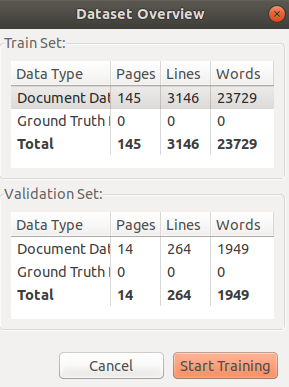
\includegraphics[width=5cm]{images/ToutLPV4datasetOverview.png}
    \label{ToutLPV4datasetOverview}
\end{figure}

La valeur de l'ensemble de validation est significative car elle montre comment le modèle se comporte sur les pages où il n'a pas été formé. Un taux de 6~\% est plutôt bon.\\

Si l'on récapitule la progression de l'entraînement du modèle, elle  s’est avérée être riche de promesses. 
\begin{itemize}
    \item Ainsi, en partant à 1849 mots, on obtenait :

CER ON TRAIN SET :~16,31 \%

CER ON VALIDATION SET : 26,25 \%
\item Puis, avec 1 951mots :

CER ON TRAIN SET~: 0,36 \%

CER ON VALIDATION SET : 27,10 \%

\item Avec 1 977 mots :

CER ON TRAIN SET : 0,29 \%

CER ON VALIDATION SET : 12,57 \%

\item Avec 4 207 mots :

CER ON TRAIN SET : 0,86 \%

CER ON VALIDATION SET : 11,55 \%

\item Avec 15 928 mots :

CER ON TRAIN SET~:~2,58 \%

CER ON VALIDATION SET : 6,40 \%

\item Avec 18 531 mots :

CER ON TRAIN SET : 2,91 \%

CER ON VALIDATION SET : 7,83 \% (même set de validation que le précédent)

\item Avec 23 729 mots :

CER ON TRAIN SET~:~3,52 \%

CER ON VALIDATION SET : 6,09 \% (même set de validation que le précédent)

\end{itemize}

Cependant, certains de ces chiffres sont biaisés car nous n'avons pas toujours utilisé le même set de validation, excepté pour les trois derniers entraînements du modèle. 

Par ailleurs, certains chiffres peuvent laisser dubitatifs car ils sont fluctuants. Cela est probablement dû à la part d’aléatoire du \emph{machine learning} en entraînement et peut-être aussi à cause de certaines images d'une qualité insuffisante.

Nous étions plutôt confiants quant aux chiffres indiquant la progression du modèle. 
En effet, si on traduit le CER en taux de réussite, nous sommes près d'un taux de réussite de 95~\% ce qui est très positif. 

Néanmoins, 5 \% de CER signifie tout de même une faute tous les 20 caractères, soit, pour une moyenne de 4 lettres par mot, 1 faute tous les 5 mots au moins.

Ceci étant établi, il est temps de voir si la réalité que cachent ces chiffres sera aussi positive qu'on l'espère : il s'agit désormais d'appliquer le dernier modèle pour que la machine opère elle-même les transcriptions. C'est l'aboutissement de notre travail. 
 
 
\section{Application du modèle}

Ayant trouvé la progression de l’entraînement du modèle plutôt bonne quant aux chiffres, nous étions assez confiante pour l’appliquer sur des manuscrits non transcrits et voir le résultat du travail d’une petite dizaine de jours.

Nous avons donc, à cette fin, mis de côté des manuscrits venant de fonds divers et variés représentant huit pages.

Pour appliquer un modèle et donc effectuer une transcription sur un manuscrit, il faut auparavant importer les manuscrits en question sur Transkribus. Puis, il faut se rendre dans l'onglet \emph{Tools} où se trouvent les outils, aller dans la partie \emph{Text recognition} et cliquer sur \inquote{Run}. Une fenêtre s'ouvre alors et l'on peut choisir les modalités de transcription et sélectionner le modèle dont on se sert pour transcrire : à chaque écriture correspond en effet un modèle adapté. Pour notre part, ayant entraîné un modèle pour l'écriture de Le Play uniquement, en toute logique, nous n'avons chargé que des manuscrits ne comportant que l'écriture de Frédéric Le Play.

Ceci fait, nous sommes allée regarder quels étaient les résultats des transcriptions automatiques. Or, pour la première page, il n'y a pas un mot sans faute, à part le « Monsieur » et la signature de Le Play. Nous avons pensé que cela était peut-être dû à la mauvaise qualité de la numérisation d'une part, et d'autre part peut-être du fait que nous n'avions entraîné pour le modèle aucune lettre de ce fonds\footnote{La première page transcrite automatiquement provient des archives départementales (AD) de Haute-Savoie, c'est une lettre de Le Play à Joseph Despine.}.

Une page est tirée du fonds de Frédéric de Mercey à la BNF. La qualité de la numérisation est donc plutôt bonne. Cependant, même si le résultat est meilleur que la précédente lettre, il reste encore beaucoup de fautes, et nous nous sommes demandée si le fait de les corriger ne prendrait pas plus de temps que de tout transcrire en partant de rien. Là encore, nous n'avions pas transcrit de lettres de ce fonds pour l’entraînement. Par ailleurs, l’écriture de Le Play varie selon son âge, et nous n'avons peut-être pas fourni de données d'entraînement comprenant toutes les périodes de la vie de Le Play. En effet, ici, l'écriture est plus fine, plus penchée, plus jeune, ce qui a peut-être posé problème pour la reconnaissance.

Une page est tirée de la bibliothèque publique universitaire de Genève~: c’est une lettre de Frédéric Le Play au père Hyacinthe Loyson. Nous avons entraîné près de 90 pages de ce fonds. Nous avons trouvé malgré cela bon nombre de fautes. D’autre part, la numérisation comportant des nuances de gris assez foncées, la machine l’a pris pour de l’écriture : cela demandera beaucoup de temps de corriger ces fautes car la machine matche à chaque fois une ligne qui n’en est pas une et croit y reconnaître de l’écriture. Il faut donc tout effacer et tout corriger.

 \begin{figure}[ht]
    \centering
    \caption{Lettre de F. Le Play au R. P. Loyson, 1870}
    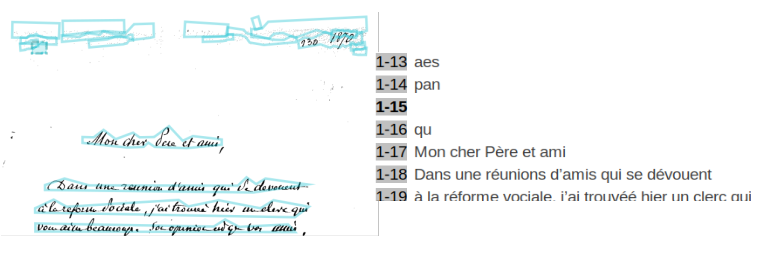
\includegraphics[width=16cm]{images/loyson.png}
    \label{loyson}
\end{figure}

Deux pages sont tirées du fonds conservé au Château de Ligoure, ce sont des lettres de Le Play à son fils Albert. La transcription est assez propre, mais subsistent encore bon nombre de fautes. Le Play forme parfois mal ses lettres, ce qui ne facilite pas la tâche, et pour l’œil humain, et pour la machine, comme nous l'avions déjà fait remarquer plus haut, ce qui d'ailleurs est aussi visible sur la figure 9.12. Par ailleurs, même si les mots sont reconnus, les accents sont souvent absents. (Par exemple, il est écrit senat pour sénat). Par ailleurs, Le Play a tendance à gommer les différences entre les majuscules et les minuscules. Souvent, ses « s » minuscules semblent être des « s » majuscules. En revanche, le « A » de « Albert » pourrait être une  minuscule, d’où de nombreuses majuscules prises pour des minuscules. 

Pour une lettre de Le Play à Alfred Tylor, le résultat est plutôt satisfaisant. La machine bute face à certains obstacles : les ratures. 

 \begin{figure}[ht]
    \centering
    \caption{Lettre de F. Le Play à Keele}
    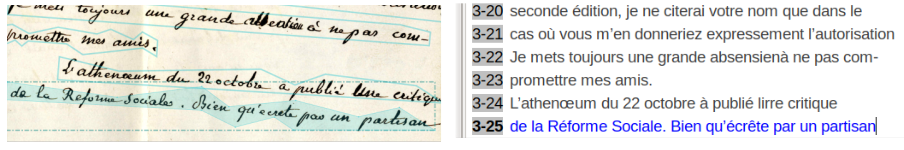
\includegraphics[width=16cm]{images/keele.png}
    \label{keele}
\end{figure}

Cependant, le résultat est plutôt bon dans l’ensemble, et la bonne qualité de la numérisation joue probablement un rôle dans ce sens. 

Pour une lettre de Le Play à Peruzzi\footnote{\emph{Biblioteca Nazionale Centrale} (Florence)
}, le résultat est plus que médiocre. Une des raisons de cet échec est la mauvaise délimitation des lignes : il y a deux sens d'écriture et la machine ne sait le reconnaître. Corriger ce genre d’erreurs prend plus de temps que de transcrire directement sans passer par la machine. Dans ce cas, il vaut mieux supprimer les lignes en question et transcrire soit-même. 

 \begin{figure}[ht]
    \centering
    \caption{Lettre de F. Le Play à Peruzzi, 1881}
    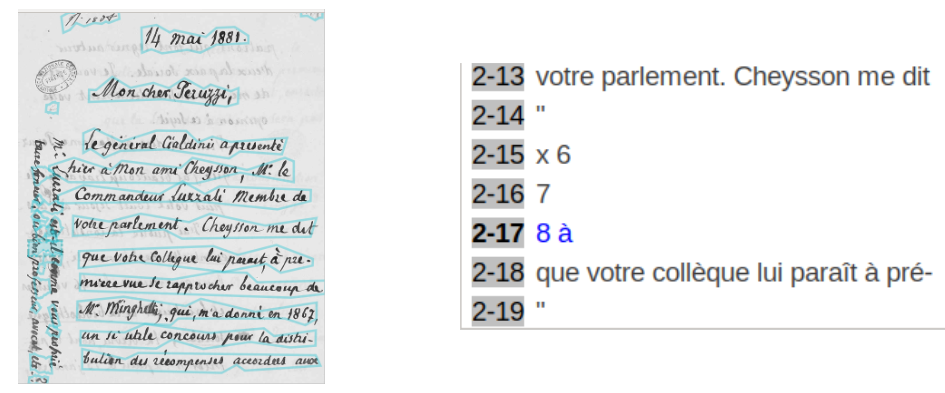
\includegraphics[width=16cm]{images/lpPeruzzi.png}
    \label{lpPeruzzi}
\end{figure}

Au terme de l'analyse de ces premières transcriptions réalisées avec notre modèle, nous avons été un peu surprise car nous pensions que les pourcentages annoncés promettaient moins de fautes.
 
Une question se pose : faut-il continuer à entraîner le modèle pour arriver à un résultat plus satisfaisant ou faut-il abandonner l’expérience ?

Deux possibilités s’ouvrent désormais : soit on entraîne encore le modèle, pour obtenir un meilleur taux de réussite, en faisant bien attention à prendre une écriture de Le Play qui couvre bien toute sa vie, car elle évolue avec le temps, (ce qui d’ailleurs nécessite d’avoir toutes les numérisations en main) et ceci avec le risque de n’avoir plus de lettres à transcrire une fois que l’on aura fini d’entraîner le modèle ; soit on laisse ainsi, mais il faudra effectuer une relecture et une correction qui risque de prendre presque autant de temps que la simple transcription : en effet, si l’on doit corriger une faute tous les cinq mots, le fait de rectifier quelque chose d’écrit pourrait prendre autant de temps que de bien transcrire directement et à la main. 

Quoi qu’il en soit, même si Transkribus n’est pas utilisé pour la transcription automatisée, avec le modèle, l’on peut toujours l’employer pour la transcription manuelle. En effet, Transkribus a le grand avantage de pouvoir être utilisé par plusieurs personnes du même projet à la fois. Ces dernières peuvent transcrire et leurs transcriptions resteront disponibles et ouvertes à toutes les personnes du groupe, ce qui permet de ne pas perdre les transcriptions dans l’ordinateur de l’un ou de l’autre. Par ailleurs, on peut ainsi mieux coller au texte, ayant le manuscrit visible sur la même page. On y trouve donc nombre d’avantages, même si l’on ne pousse pas la machine jusqu’au bout de ses capacités. Transkribus est un excellent outil de transcription collaborative qui permet d'avoir l'image et sa transcription en vis-à-vis ce qui est très confortable pour transcrire, même manuellement. 

Par ailleurs Le Play a une correspondance dont le nombre de lettres varie selon les correspondants, et si la majorité des lettres dont nous disposons sont écrites de sa main, beaucoup sont également des lettres passives. Certaines sont nombreuses, comme celles par exemple de Napoléon-Joseph Bonaparte\footnote{On dénombre 98 lettres de Napoléon-Joseph Bonaparte à Frédéric Le Play.}, mais d’autres sont rares, comme celles de Louis-Joseph Buffet\footnote{Louis-Joseph Buffet n’adresse que deux lettres à Le Play. }. 

Reste enfin la question de l’export des données, une fois que les transcriptions ont été réalisées, pour les encoder en vue de l’édition numérique de correspondance qui est tout l’objet de notre projet.


\section{Rester maître de ses données}

\subsection{Exportation en vue de l'édition}

Une fois que les transcriptions sont réalisées, il s'agit de les exporter. En effet, si elles sont toutes conservées dans le serveur de Transkribus, cela ne signifie pas que nous les avons dans nos serveurs propres. Il s'agit donc d'exporter les données pour les conserver au CRHXIX et rester maître des données : nous ne savons pas comment Transkribus va évoluer, si l'outil deviendra payant ou ne sera plus maintenu, il est donc important d'assurer ses données. 

Il faudrait penser également à la question du stockage des données, mais nous n'avons pas eu à la traiter durant notre stage, cela se fera par la suite. \\

Une question surtout se pose : comment exporter les données ? Plusieurs formats sont disponibles : \inquote{le package complet comprenant les fichiers image d'origine, les fichiers XML et les métadonnées ajoutés au document, un PDF (avec le texte transcrit inclus), doc et TEI. Tous les fichiers sont stockés dans un dossier\footnote{Régis Schlagdenhauffen, \emph{Comment utiliser Transkribus en 10 étapes (voire moins)}, Site web de l'EHESS, URL~: \url{http://regis-schlagdenhauffen.eu/wp-content/uploads/2018/01/Comment-utiliser-Transkribus-\%E2\%80\%93-en-10-\%C3\%A9tapes-ou-moins.pdf} (visité le 22/05/2020).)}}.

En vue de notre édition numérique de correspondance, nous avons exploré les différents formats d'exportation possibles. Les formats TXT et TEI s'avèrent être particulièrement intéressants. 
Lequel des deux privilégier ? 
Pour cela, il s'agit de considérer de plus près la question des \emph{tags} dans Transkribus.

\subsection{La question des \emph{tags}}

Dans Transkribus, on peut déjà caractériser certains mots grâce à des \emph{tags}. Nous avons pensé dans un premier temps utiliser les \emph{tags}\footnote{\inquote{Un tag (ou étiquette, marqueur, libellé) est un mot-clé (signifiant) ou terme associé ou assigné à de l'information [...], qui décrit une caractéristique de l'objet et permet un regroupement facile des informations contenant les mêmes mots-clés}. Voir \emph{Tag (métadonnée)}, Wikipédia, URL : \url{https://fr.wikipedia.org/wiki/Tag_(m\%C3\%A9tadonn\%C3\%A9e)} (visité le 26/09/2020).} de Transkribus, afin d'annoter en direct nos données. 

De nombreux \emph{tags} sont disponibles dans Transkribus\footnote{Voir les annexes, B.3 : Schématisation du modèle d'information de Transkribus.}. 
Nous nous sommes donc livrée à cette expérience et avons constaté que l'annotation des \emph{tags} dans Transkribus prenait beaucoup de temps. L'exemple de la figure 9.15 ci-dessous illustre les 21 \emph{tags} que nous avons mis pour une seule page de manuscrit.

 \begin{figure}[ht]
    \centering
    \caption{Pour une page, 21 \emph{tags}}
    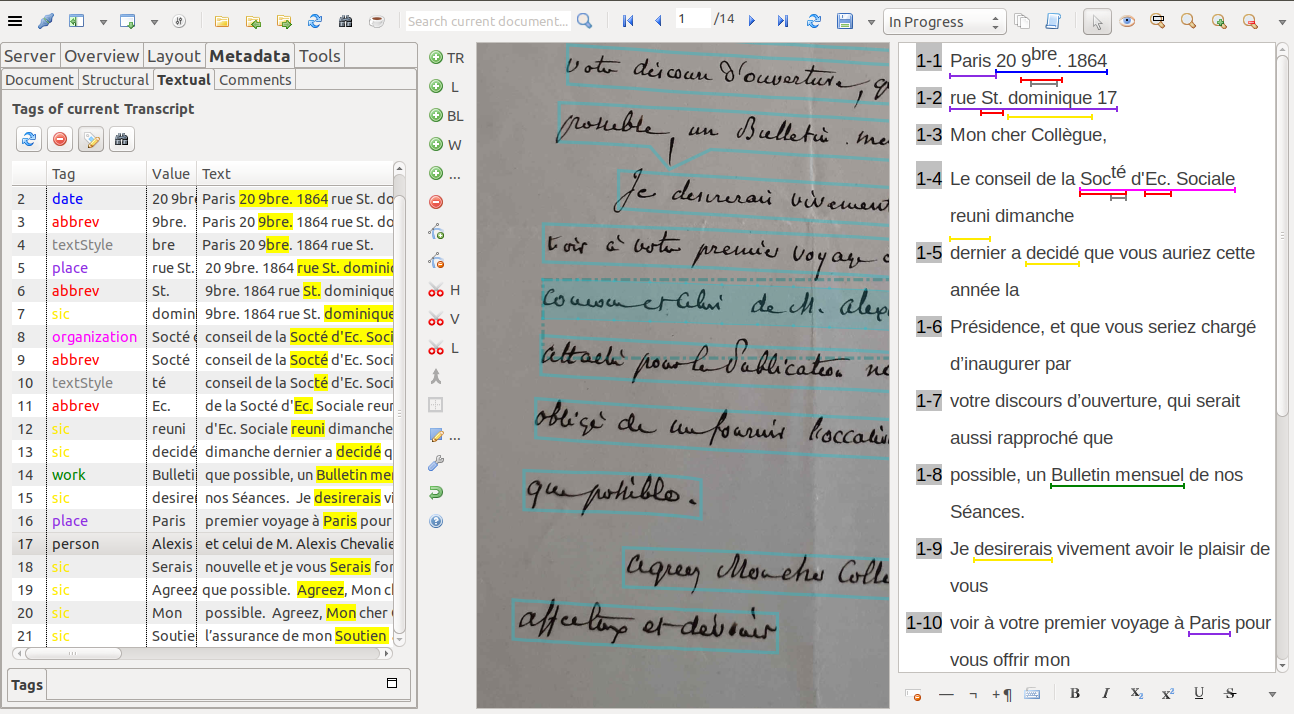
\includegraphics[width=16cm]{images/21tagTranskribus.png}
    \label{21tagTranskribus}
\end{figure}

En l'occurence, sur cette page, nous avons mentionné la date (\emph{date}), les abréviations (\emph{abbrev}), les exposants (\emph{textStyle)}), les noms de lieu (\emph{place}), les fautes dans l'original (\emph{sic}), les noms d'organisation (\emph{organization}), les noms d'ouvrage (\emph{work}), les noms de personne (\emph{person}).

L'avantage de renseigner en amont ces informations permet, lors de l'export, de les retrouver directement dans nos fichiers en XML-TEI. 
Cependant, nous n'avons pas opté pour ce choix pour plusieurs raisons : 
\begin{itemize}
    \item Nous avons été mise en garde sur l'export en TEI qui n'est pas encore tout à fait au point dans Transkribus
    \item Nous avons pris connaissance trop tard du guide d'utilisation des \emph{tags} dans Transkribus et de la possibilité de personnaliser ses propres \emph{tags}\footnote{\emph{How to enrich transcribed documents with mark-up}, \url{https://transkribus.eu/wiki/images/e/e8/How_to_enrich_transcribed_documents_with_mark-up.pdf} (visité le 26/09/2020).}.
    \item Nous aurions de toutes façons manqué de temps pour penser les \emph{tags} dans Transkribus à long terme
    \item L'export des \emph{tags} déjà existant s'est avéré être non conforme pour la TEI et nous avons dû corriger nombre de noms de balises.
    Nous aurions pu passer par une feuille de transformation (XSLT : \emph{eXtensible Stylesheet Language Transformations}) permettant de passer du fichier TEI exporté à un fichier TEI comportant les noms de balises que nous voulons mettre, mais ceci nécessite une bonne maîtrise de la technologie et nous pensons qu'il est préférable d'apprendre d'abord à l'équipe du CRHXIX à maîtriser XML au lieu de passer directement à la maîtrise d'XSLT. 
    \item Enfin et surtout, nous avons préféré penser le balisage directement dans XML-TEI. 
\end{itemize}

Quoi qu'il en soit, nous n'excluons pas pour le CRHXIX d'utiliser l'interface graphique de Transkribus pour les \emph{tags}. Il suffira à la personne qui prendra la suite de la partie numérique du projet de penser la chose. Nous avons de notre côté pensé surtout à l'enchaînement des balises.\\


L'export en TEI est tout de même intéressant pour ce qui est de la structure du texte (une balise délimite les lignes ce qui est intéressant). On peut également opter pour un export en TXT étant donné que la délimitation des lignes est également respectée. \\

Nous voyons que la phase d'acquisition des données s'est avérée riche en questionnements. L'apprentissage machine a eu une large part dans cette partie de nos stages, aussi bien pour l'OCR de Gallica que pour l'HTR de Transkribus. Que ce soit pour l'OCR ou l'HTR, nous n'en sommes pas encore à du 100~\% quant au résultat, néanmoins, ces technologies nous ont été d'un grand secours. La part de relecture reste tout de même importante. \\

Une fois les données acquises, il s'agit de les traiter en vue de leur valorisation et donc de leur mise en ligne. 
Qu'en est-il du traitement des données pour l'édition numérique de correspondance ? 
C'est l'objet de notre dernière partie.

